\ifdefined\ishandout
\documentclass[handout]{beamer}
\else
\documentclass{beamer}
\fi

%\usepackage[frenchb]{babel}
\usepackage[T1]{fontenc}
%\usepackage[utf8]{inputenc}
\usepackage{hyperref}
\usepackage{multirow}
\usepackage{listings}
\usepackage{fancyvrb}
\usepackage{tikz}
\usepackage{framed}
\usepackage{xmpmulti}
\usepackage{algorithm}
\usepackage{algorithmicx}
\usepackage{algpseudocode}
\usepackage{xcolor}
\usepackage{booktabs}
\usepackage{color, colortbl}
\ifdefined\ishandout
\usepackage{handoutWithNotes}
\fi
\usepackage{slashbox}
\usepackage{amsmath}
\usepackage{bm}
\usepackage{hhline}
\usepackage{pgfplots}
\usepackage{caption}

\def\UrlBreaks{\do\/\do-}

\usetikzlibrary{shapes.geometric}
\usetikzlibrary{positioning}
\usetikzlibrary{shapes.arrows, chains}
\usetikzlibrary{arrows,calc}
\usetikzlibrary{shapes.multipart}
\usetikzlibrary{matrix}

\usepackage{array}
%\usetheme{Boadilla}
\usetheme[progressbar=frametitle]{metropolis}

\usefonttheme[onlymath]{serif}

\newcommand{\R}{\mathbb{R}}
%\newcommand{\C}{\mathbb{C}}
\newcommand{\N}{\mathbb{N}}
\newcommand{\Z}{\mathbb{Z}}
\newcommand{\E}{\mathbb{E}}
\newcommand{\Var}{\text{Var}}
\newcommand{\Cov}{\text{Cov}}
\ifdefined\ishandout
\pgfpagesuselayout{3 on 1 with notes}[a4paper,border shrink=5mm]
\usecolortheme{dove}
\else
%\usecolortheme{dolphin}
%\usecolortheme{crane}
\fi

\metroset{block=fill}

\lstnewenvironment{codeC}
{ \lstset{language=C,
    otherkeywords={printf,scanf}}
}
{}

\ifdefined\ishandout
\definecolor{mygreen}{rgb}{0,0,0}
\definecolor{mymauve}{rgb}{0,0,0}
\definecolor{myblue}{rgb}{0,0,0}
\else
\definecolor{mygreen}{rgb}{0,0.6,0}
\definecolor{mymauve}{rgb}{0.58,0,0.82}
\definecolor{myblue}{rgb}{0,0,1}

\fi

%% Notes
%\setbeameroption{show only notes}


\definecolor{mygray}{rgb}{0.5,0.5,0.5}

\lstset{ language=Python,%
  backgroundcolor=\color{white},   % choose the background color; you must add \usepackage{color} or \usepackage{xcolor}
  basicstyle=\footnotesize,        % the size of the fonts that are used for the code
  breakatwhitespace=false,         % sets if automatic breaks should only happen at whitespace
  breaklines=true,                 % sets automatic line breaking
  captionpos=b,                    % sets the caption-position to bottom
  commentstyle=\color{mygreen},    % comment style
  deletekeywords={...},            % if you want to delete keywords from the given language
  escapeinside={\%*}{*)},          % if you want to add LaTeX within your code
  extendedchars=true,              % lets you use non-ASCII characters; for 8-bits encodings only, does not work with UTF-8
  frame=tb,	                   % adds a frame around the code
  keepspaces=true,                 % keeps spaces in text, useful for keeping indentation of code (possibly needs columns=flexible)
  keywordstyle=\color{blue},       % keyword style
  otherkeywords={*,...},           % if you want to add more keywords to the set
  numbers=none,                    % where to put the line-numbers; possible values are (none, left, right)
  numbersep=5pt,                   % how far the line-numbers are from the code
  numberstyle=\tiny\color{mygray}, % the style that is used for the line-numbers
  rulecolor=\color{black},         % if not set, the frame-color may be changed on line-breaks within not-black text (e.g. comments (green here))
  showspaces=false,                % show spaces everywhere adding particular underscores; it overrides 'showstringspaces'
  showstringspaces=false,          % underline spaces within strings only
  showtabs=false,                  % show tabs within strings adding particular underscores
  stepnumber=2,                    % the step between two line-numbers. If it's 1, each line will be numbered
  stringstyle=\color{mymauve},     % string literal style
  tabsize=3,	                   % sets default tabsize to 2 spaces
  title=\lstname                   % show the filename of files included with \lstinputlisting; also try caption instead of title
}
%\lstset{language=Python,
% breakatwhitespace=false,         % sets if automatic breaks should only happen at whitespace
%  breaklines=true,                 % sets automatic line breaking
%  captionpos=b,                
%%commentstyle=\itshape\color{mymauve},
%%keywordstyle=\bfseries\color{myblue},
%numbers=left,                    % where to put the line-numbers; possible values are (none, left, right)
%  numbersep=8pt,                   % how far the line-numbers are from the code
%  numberstyle=\tiny\color{mygray}, % the style that is used for the line-numbers
%%  rulecolor=\color{black},         % if not set, the frame-color may be changed on line-breaks within not-black text (e.g. comments (green here))
%  showspaces=false,                % show spaces everywhere adding particular underscores; it overrides 'showstringspaces'
%%  showstringspaces=false,          % underline spaces within strings only
%  showtabs=false,                  % show tabs within strings adding particular underscores
%  stepnumber=2,                    % the step between two line-numbers. If it's 1, each line will be numbered
%%  stringstyle=\color{mygreen},     % string literal style
%  tabsize=2 
%}
\ifdefined\ishandout
\newcommand{\red}{\textbf}
\else
\newcommand{\red}{\textcolor{red}}
\fi
%\newcommand \emph
%Default size : 12.8 cm * 9.6 cm

\newcommand{\tmark}[1]{\tikz[remember picture, baseline=-.5ex]{\coordinate(#1);}}

\definecolor{bluegreen}{RGB}{0,149,182}


%\newcommand{\output}[1]{
\setbeamertemplate{navigation symbols}{}
\newcommand{\bvrb}{\Verb[commandchars=£µ§,formatcom=\color{bluegreen}]}
\newcommand{\footvrb}{\footnotesize\Verb}
\newcommand{\vrbalert}[2][]{\visible<#1>{#2}}
%%% Commande pour les listes/arbres
\newcommand{\mvide}{\nodepart{one} \nodepart{two}}
\newcommand{\tvide}{\nodepart{one} \nodepart{two} \nodepart{three}}
\newcommand{\rref}[1][]{\hfill{\scriptsize\textit{#1}}}

%%Fin des commandes pour les listes/arbres.



%%% Paramètres du cours (à régler)
%Numéro du cours
\newcommand{\nb}{1}

\title[Machine Learning]{Machine learning and physical (Earth system) modelling}
\author[J. Brajard]{julien.brajard@nersc.no}
\institute[NERSC]{NERSC\\
slides:\url{https://github.com/nansencenter/crash-course-ML-slides}\\
notebooks: \url{https://github.com/nansencenter/ml-crashcourse}}
\date{June 2021}

\begin{document}
%%%%%%%%%%%%%%%%%%%%% SLIDES DE TITRE
\begin{frame}
\titlepage
\end{frame}



%%%%%%%%%%%%%%%%%%%%%
\begin{frame}{References}
    \bibliographystyle{alpha}
    \nocite{Goodfellow-et-al-2016,VanderPlas-2016}
\bibliography{myref.bib}
\end{frame}

\begin{frame}{Table of contents}
  \setbeamertemplate{section in toc}[sections numbered]
  \tableofcontents[hideallsubsections]
\end{frame}




\section{Introduction}

%%%%%%%%%%%%%%%%%%%%%
\begin{frame}{Scope of the lecture: Machine Learning}
%\centering
%  \begin{tikzpicture}[scale=0.9]
%    \draw<3-> {(0,0) ellipse (2 and 1)};
%    \draw<2-> {(0.3,0.3) ellipse (2.5 and 1.5)};
%    \draw<1-> {(0.6,0.6) ellipse (3.1 and 2.1)};
%    \draw<5->[line width = 0.5mm]  {(0.3,0.3) ellipse (2.5 and 1.5)};
%     \node<3-> at (0,0) {Deep Learning};
 % \node<2-> at (.3,1.2) {\alert<5->{Machine Learning}};
 % \node<1-> at (0.7,2) {Artificial intelligence};
 % \end{tikzpicture}  
 \begin{center}
     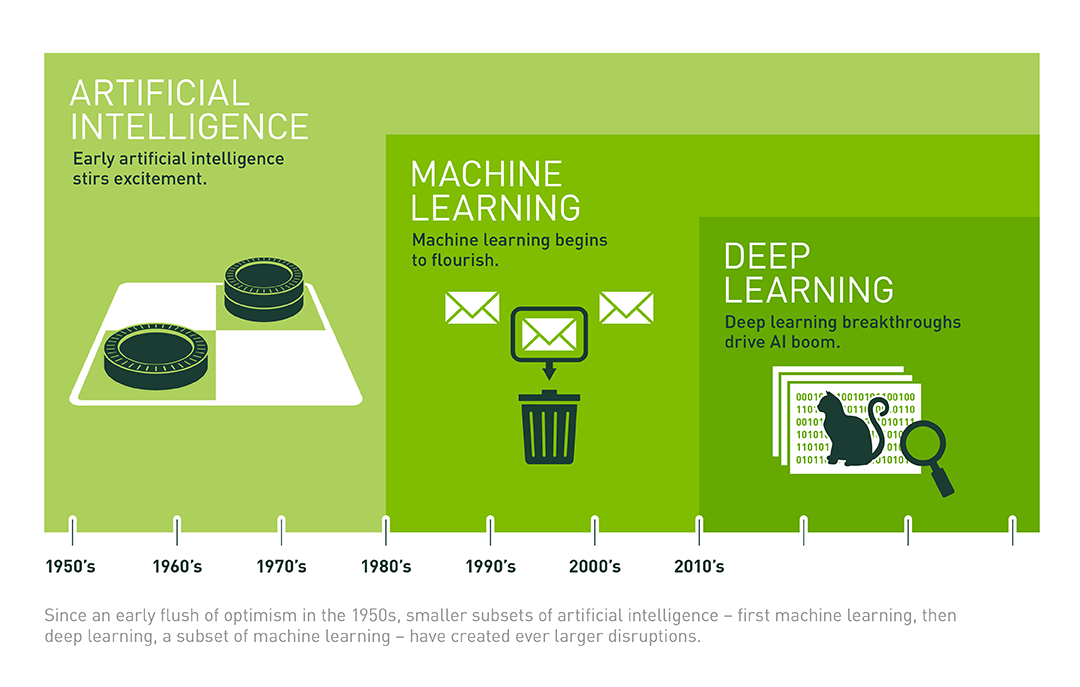
\includegraphics[width=\textwidth]{fig/L1/Deep_Learning_Icons_R5_PNG.png}
 \end{center}
 \rref[Source: NVidia]
 \end{frame}
 \begin{frame}{A (very) active field}
\begin{columns}
\column{.5\textwidth}
\begin{figure}
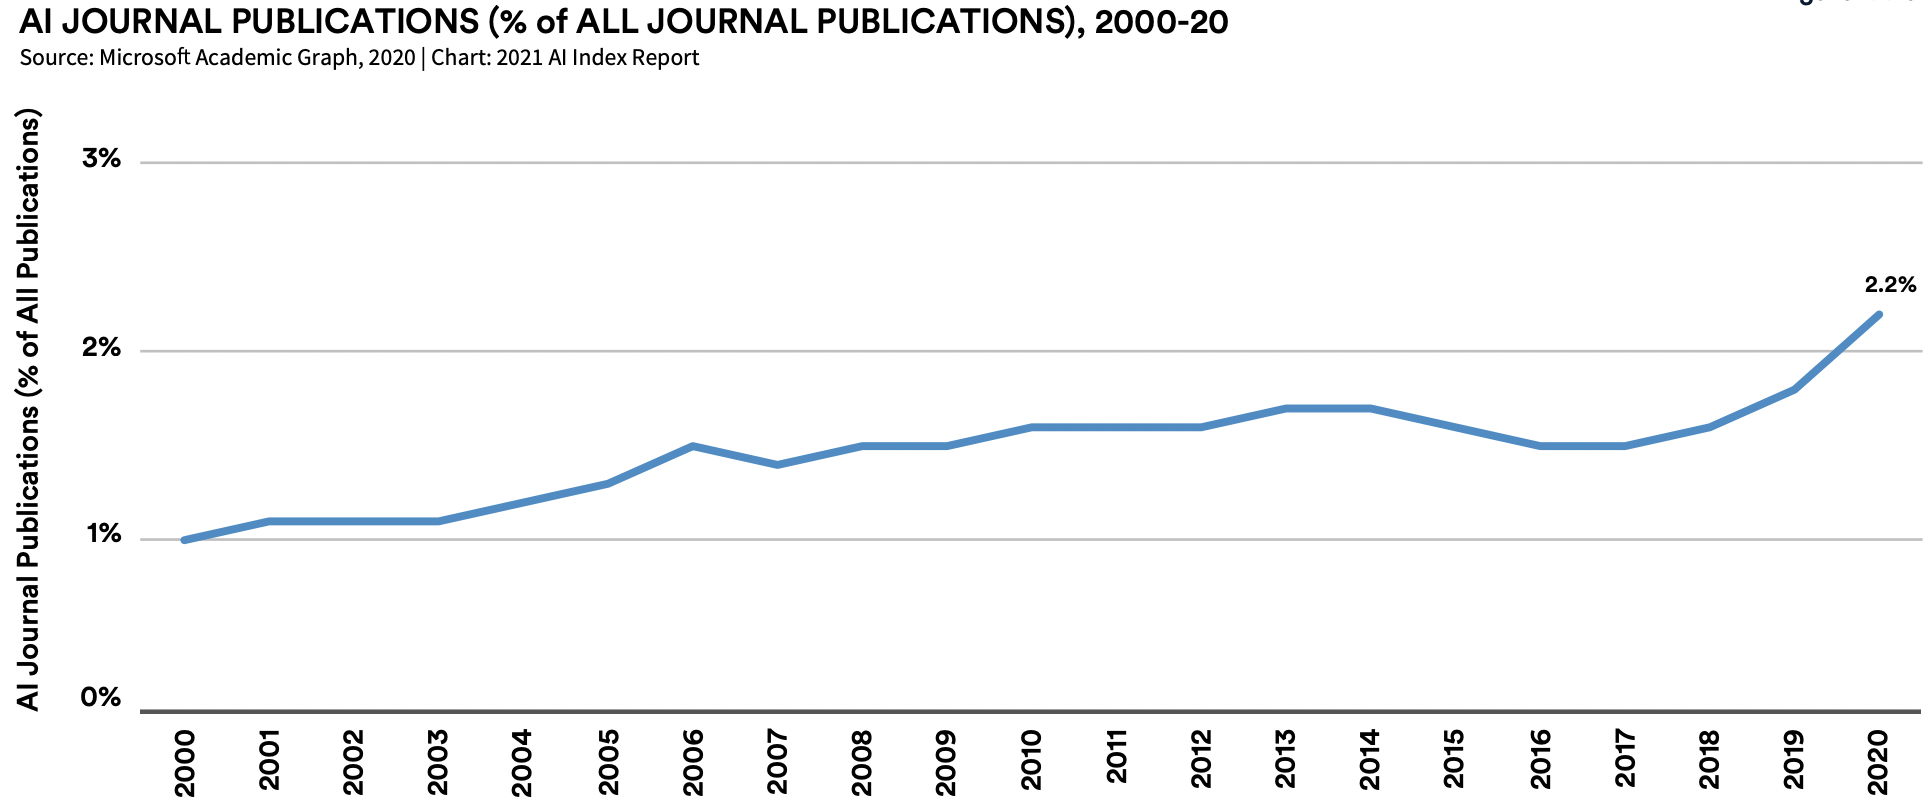
\includegraphics[width=\textwidth]{fig/L1/progress-papers.png}
\end{figure}
\column{.5\textwidth}

\begin{figure}
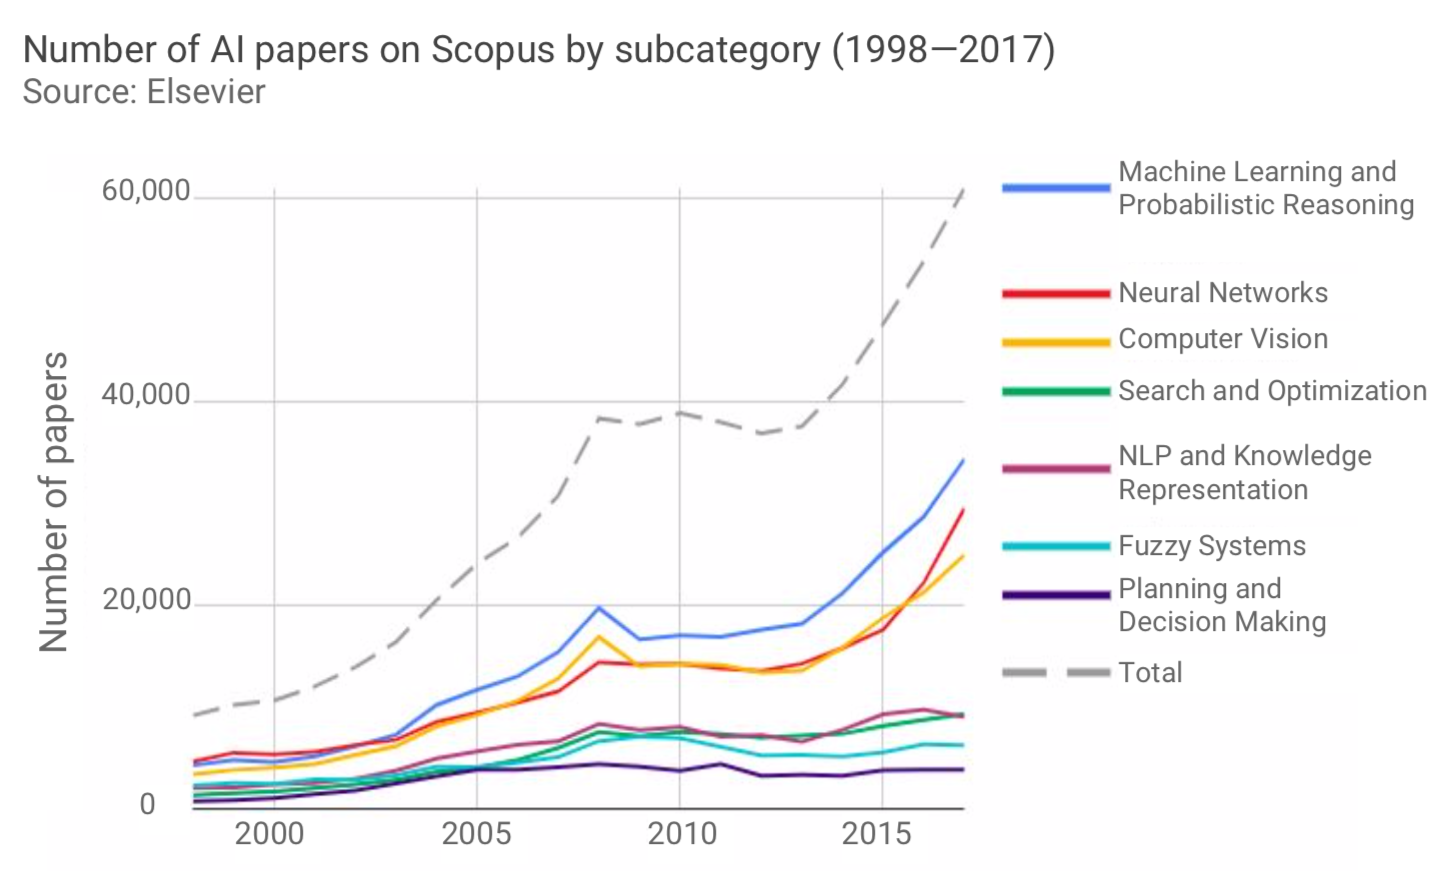
\includegraphics[width=\textwidth]{fig/L1/progress-ml.png}
\end{figure}
  \end{columns}
  \rref[Shoham et al., AI Index 2018 Annual Report]

\end{frame}



%%%%%%%%%%%%%%%%%%%%
\begin{frame}
\frametitle{Example 1: Computer Vision}
\begin{figure}
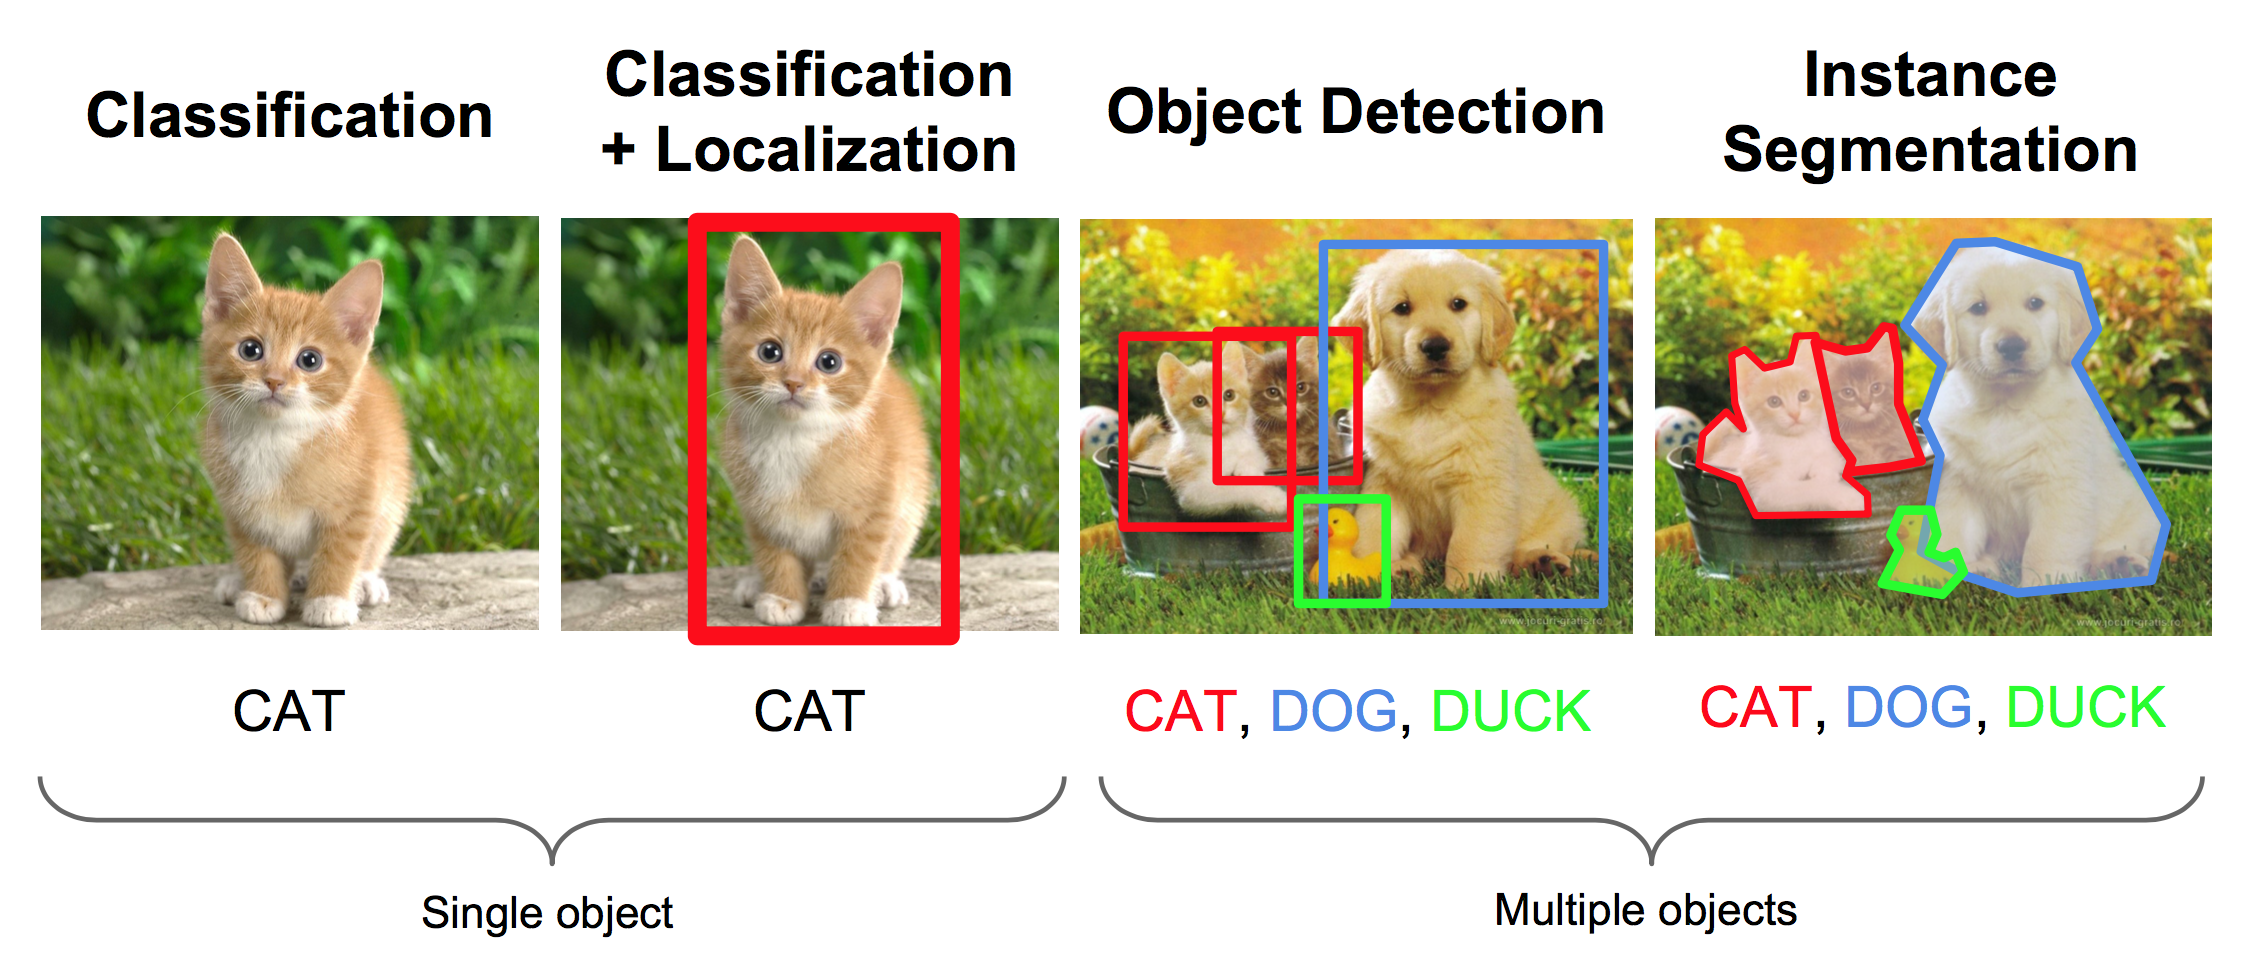
\includegraphics[width=\textwidth]{./fig/L1/compute-vision.png}
\end{figure}
\rref[Li, Karpathy and Johnson, 2016, Stanford CS231n course]

\end{frame}


%%%%%%%%%%%%%%%%%%%%
\begin{frame}
\frametitle{Example 1: Computer Vision}
\framesubtitle{Image Net Large Scale Recogonition Challenge (ILSVRC)}
\begin{figure}

\begin{tikzpicture} [scale=0.8, every node/.style={scale=0.6}]
  \begin{axis}[ 
    x tick label style={ 
      /pgf/number format/1000 sep=}, 
    ylabel=Classification error, 
    xtick={2010,2011,2012,2013,2014,2015,2016,2017},
    xticklabels={2010,2011,2012,2013,2014,2015,2016,hum.},
    enlargelimits=0.15, 
     bar width=7pt, 
    ybar,
   legend style={at={(0.5,-0.15)},
     anchor=north,legend columns=-1}, 
   x tick label style={font=\footnotesize,rotate=45, anchor=east},
   very axis plot/.append style={
      ybar,
      bar width=.2,
      bar shift=0pt,
      fill},
      nodes near coords,
   ] 
   \addplot[ybar,fill=blue!60, bar shift=0pt]
   coordinates {(2010,28) (2011,26)}; 
   \addplot[ybar,fill=red!60]
   coordinates {(2012,16) (2013,12) (2014,7) (2015,3.6) (2016,3)}; 
   \addplot[ybar,fill=green!60, bar shift=0pt] 
   coordinates 
   {(2017,5.1)};  
   \legend{traditional algo.,Deep Learning,Human}
 \end{axis} 
\end{tikzpicture}
\end{figure}
Deep learning architectures were based on Convolutional Neural Networks (CNN).
\end{frame}



%%%%%%%%%%%%%%%%%%%%
\begin{frame}
\frametitle{Example 2: Machine Translation}
Objective : translate a text from a language to another.
\begin{figure}

\includegraphics[width=.8\textwidth]{./fig/L1/google-trad.png}
\end{figure}
\begin{itemize}
\item {\bf Oct. 2013}: Pionneering scientic paper about neural networks in machine translation (Kalchbrenner, N., and Blunsom, P).
\item {\bf 2016}: Neural machine translation outperform tradiational approaches on public benchmarks
\item {\bf 2017}: Major systems (Google, Systran, WIPO, Microsoft) switch to
  neural machine translation  (using deep recurrent neural networks)
\end{itemize}
\end{frame}


%%%%%%%%%%%%%%%%%%%%
\begin{frame}
\frametitle{Example 3: Playing Games}
\begin{columns}
\column{.5\textwidth}
\begin{itemize}
\item {\bf 1997}: Deep Blue defeats Kasparov at Chess.
\item {\bf 2016}: AlphaGo's victory again Lee Sedol at Go.
\item {\bf 2017}: AphaGo Zero learns how to play Go only by playing against
  itself. It outperformed previous AlphaGo version (Reinforcement
  learning)
\item {\bf 2017}: DeepStack beats professional human poker players.
\end{itemize}
\column{.5\textwidth}
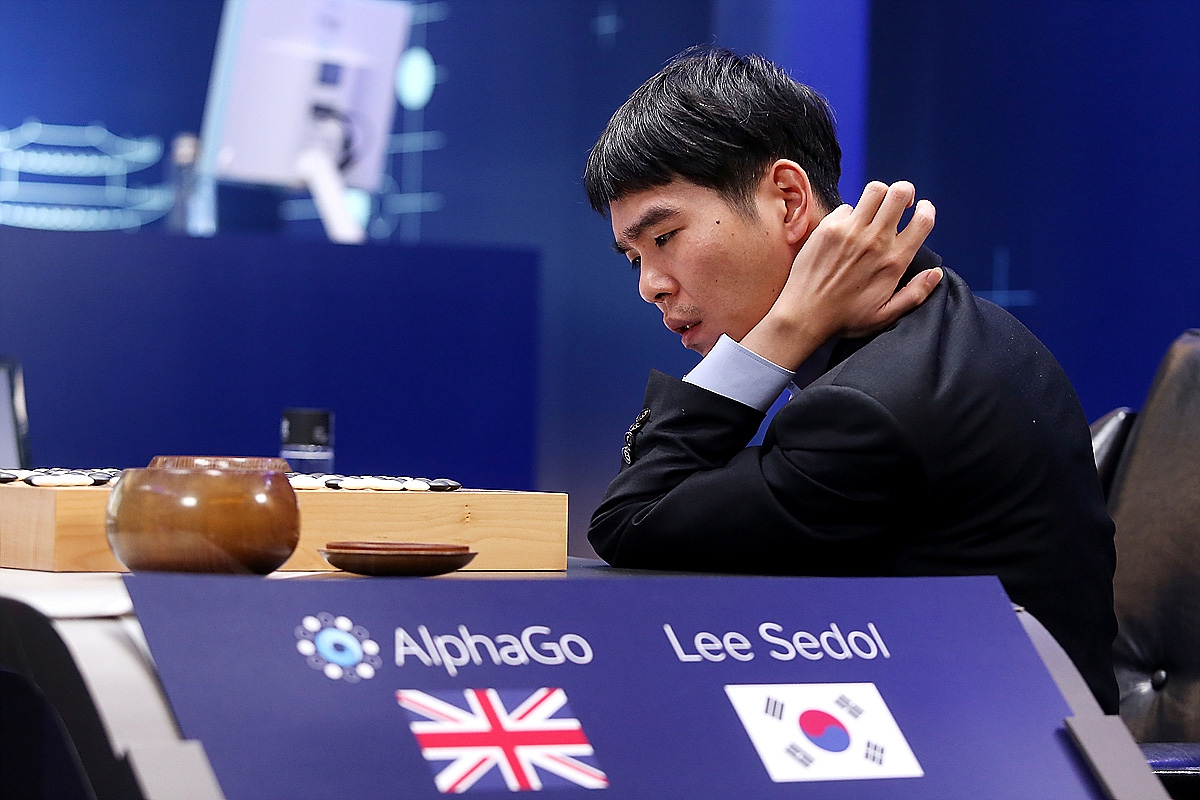
\includegraphics[width=\textwidth]{./fig/L1/alphago.jpg}
\end{columns}
\end{frame}

%%%%%%%%%%%%%%%%%%%%%
\begin{frame}{Predicting sport results?}
Rugby World Cup 2019
   \begin{figure}
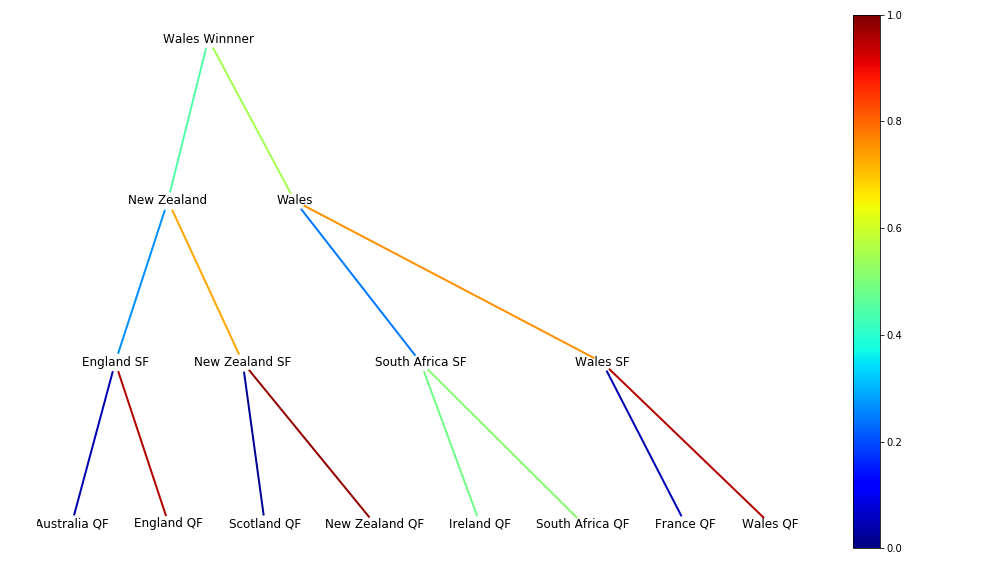
\includegraphics[width=.9\textwidth]{fig/L1/predicting-rugby.png} 
\end{figure}
Prediction based on XGBoost.
\begin{scriptsize}
   \url{https://towardsdatascience.com/predicting-the-winner-of-the-rugby-world-cup-2019-89a27d3f5b8e}
\end{scriptsize}

\end{frame}

\begin{frame}{AI Art?}
    \begin{figure}
        \centering
        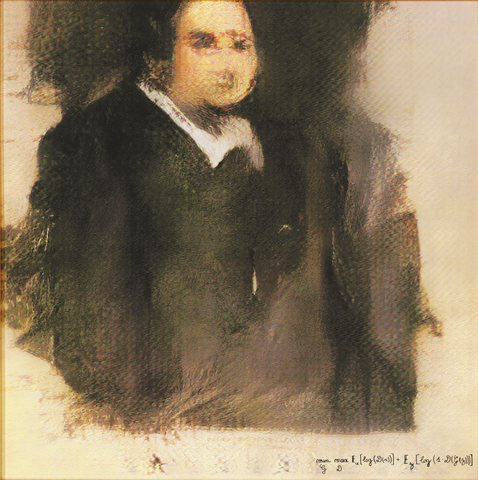
\includegraphics[width=0.5\textwidth]{fig/L3/478px-Edmond_de_Belamy.png}
        \caption*{\textit{Edmond de Bellamy} by Obvious(collective)}
    \end{figure}
    Generated using a Generative Adversarial Network.\\
    Selling prince (Oct. 2018): \$432,000
\end{frame}


%%%%%%%%%%%%%%%%%%%%%%%%
\begin{frame}[t]{Reasons for these recent achievements?}
    \begin{itemize}
        \item Increasing of the datasets in size and quality
        \only<1> {
        \begin{figure}
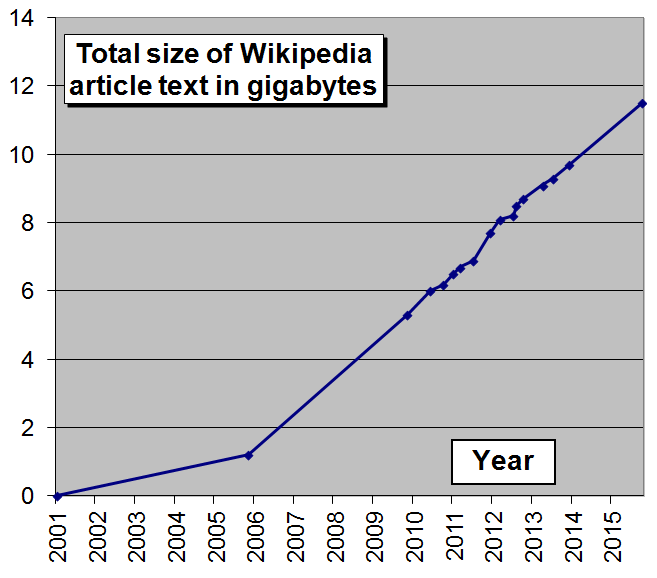
\includegraphics[width=.6\textwidth]{fig/L1/Wikipedia_article_size_in_gigabytes.png}
\end{figure}
\rref[source: Wikipedia]
}
        \item <2-> Progress in computing resources.
        \only<2> {
        \begin{figure}
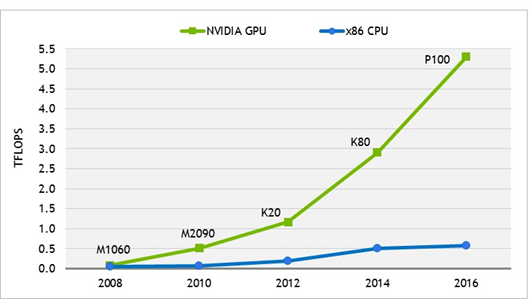
\includegraphics[width=.7\textwidth]{fig/L1/evolution-gpu.png}
\end{figure}
\rref[source: NVDIA]
}        
        
        \item <3-> Scientific research on new algorithms (e.g adapted to image processing)
                \only<3> {
        \begin{figure}
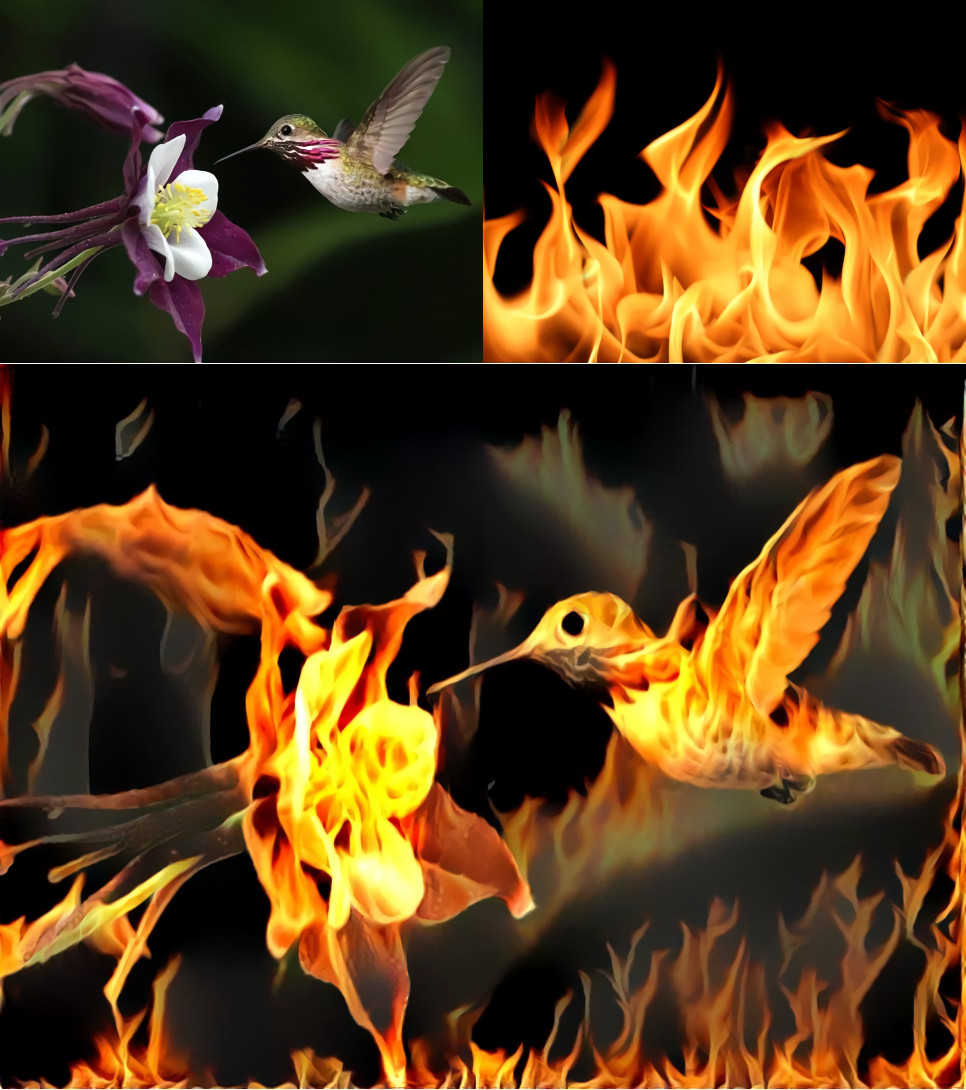
\includegraphics[width=.4\textwidth]{fig/L1/deep-art.jpg}
\end{figure}
\rref[source: Deep Dream Generator]

}        
    \end{itemize}

\end{frame}

\begin{frame}{Apply Machine-Learning to physical modelling?}
\alert{Why is it a good idea?}
    \begin{itemize}
        \item A increasing number of geophysical data (one spatial mission: 24 TB/day)
          \only<1> {
        \begin{figure}
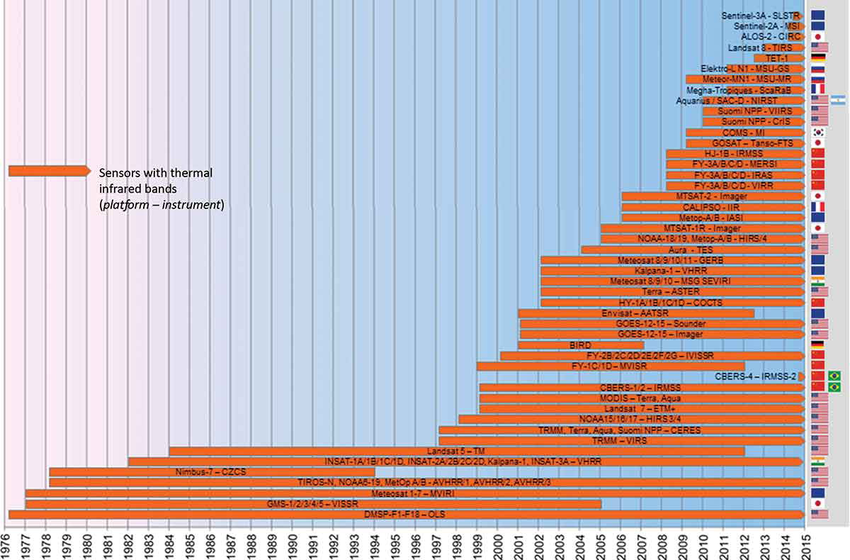
\includegraphics[width=.55\textwidth]{fig/L1/sat-sst.png}
\caption*{Satellites providing a semi-global daily coverage of surface temperature}
\end{figure}
\rref[source: Kuenzer et al. (2014)]
}
        \item <2->Data with highly significant spatial patterns
                  \only<2> {
        \begin{figure}
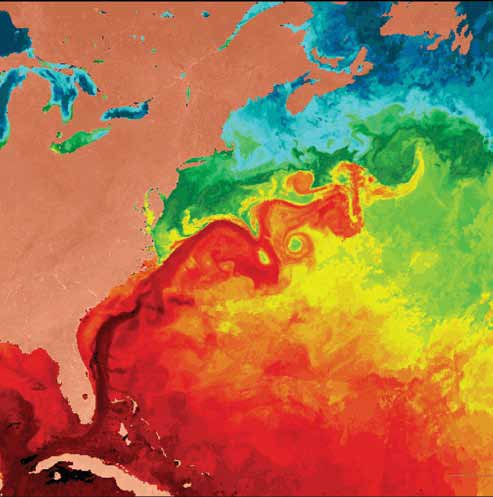
\includegraphics[width=.36\textwidth]{fig/L1/Satellite-image-of-sea-surface-temperature-showing-the-gulf-Stream-and-large-rings-and_W640.jpg}
\caption*{Sea Surface temperature of the gulf stream}
\end{figure}
\rref[source: Talley (2000)]
}
    \end{itemize}
\end{frame}

\begin{frame}{Why is physical modelling specific?}

\begin{columns}


\column{.5\textwidth}
\begin{figure}
    \caption*{NASDAQ Composite sock market index over the last 10 years}
    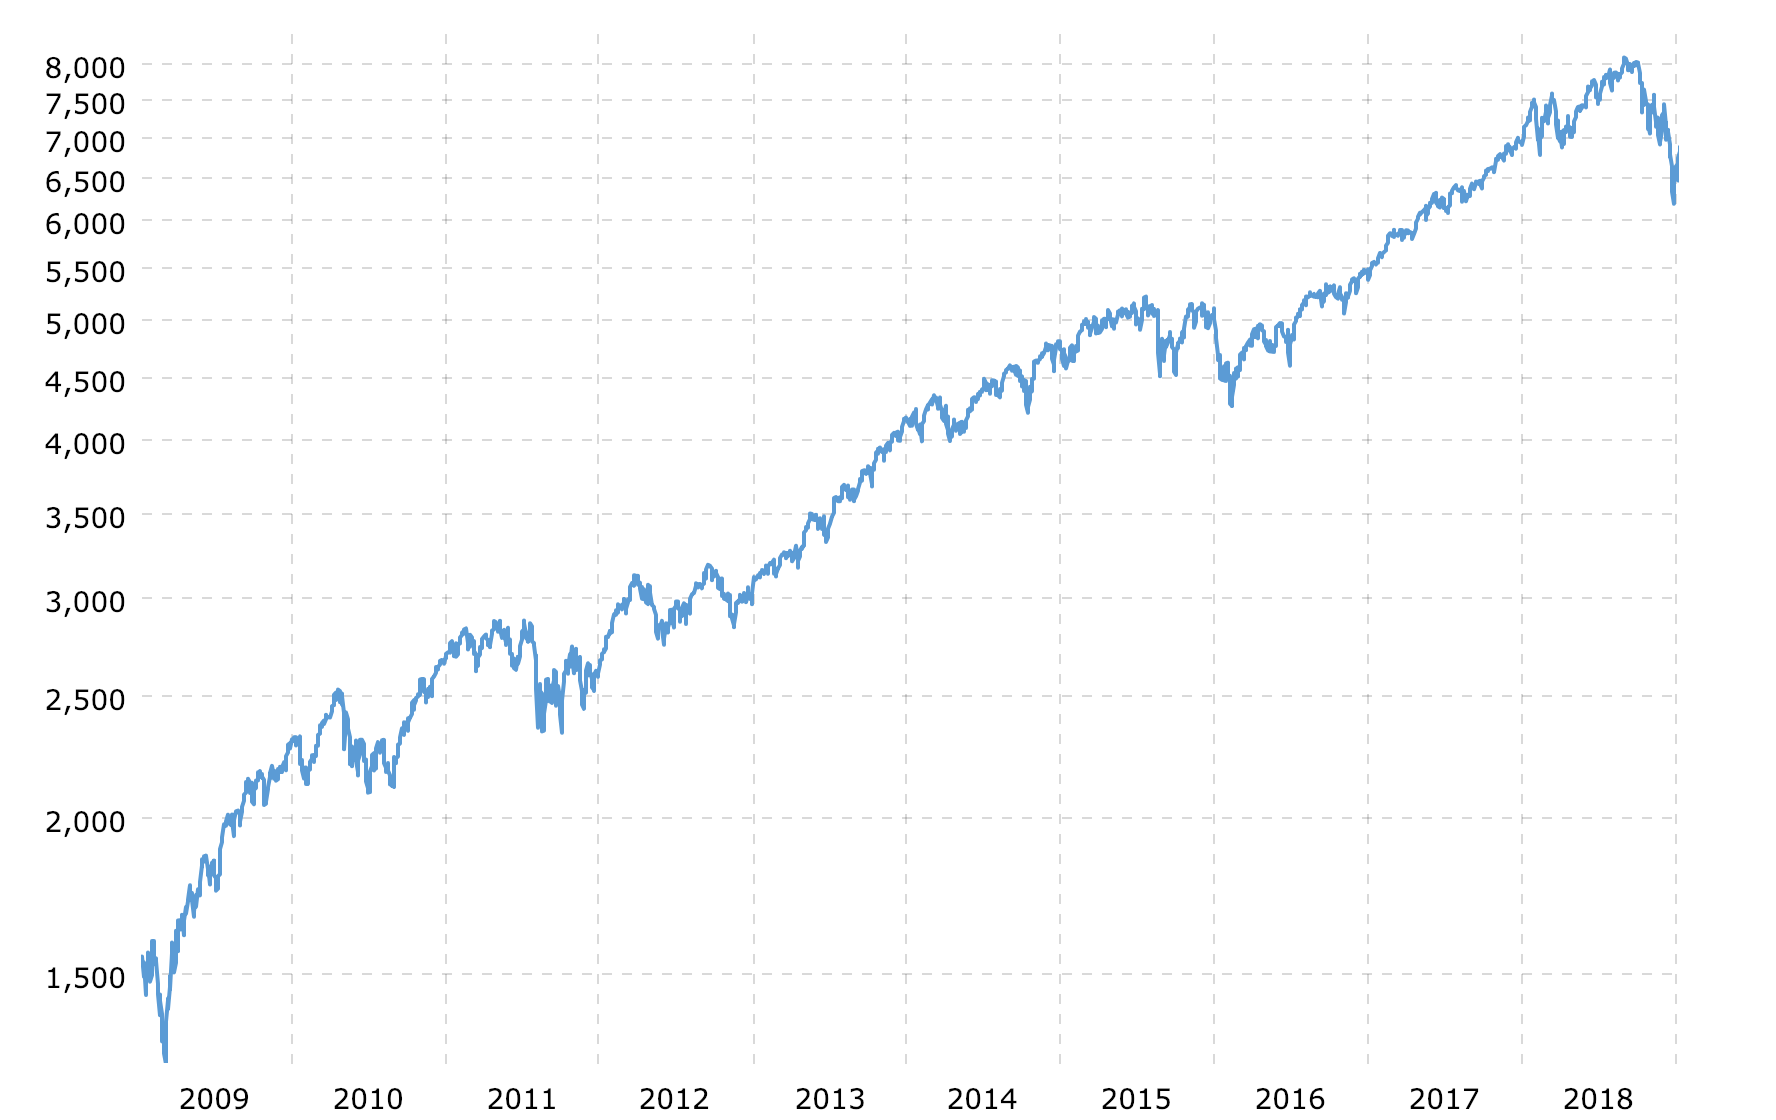
\includegraphics[width=\textwidth]{fig/L1/nasdaq-composite-index-10-year-daily-chart-2019-01-09-macrotrends.png}
\end{figure}
\visible<2->{\alert{Mostly unknown dynamical processes}}

\column{.5\textwidth}
\begin{figure}
    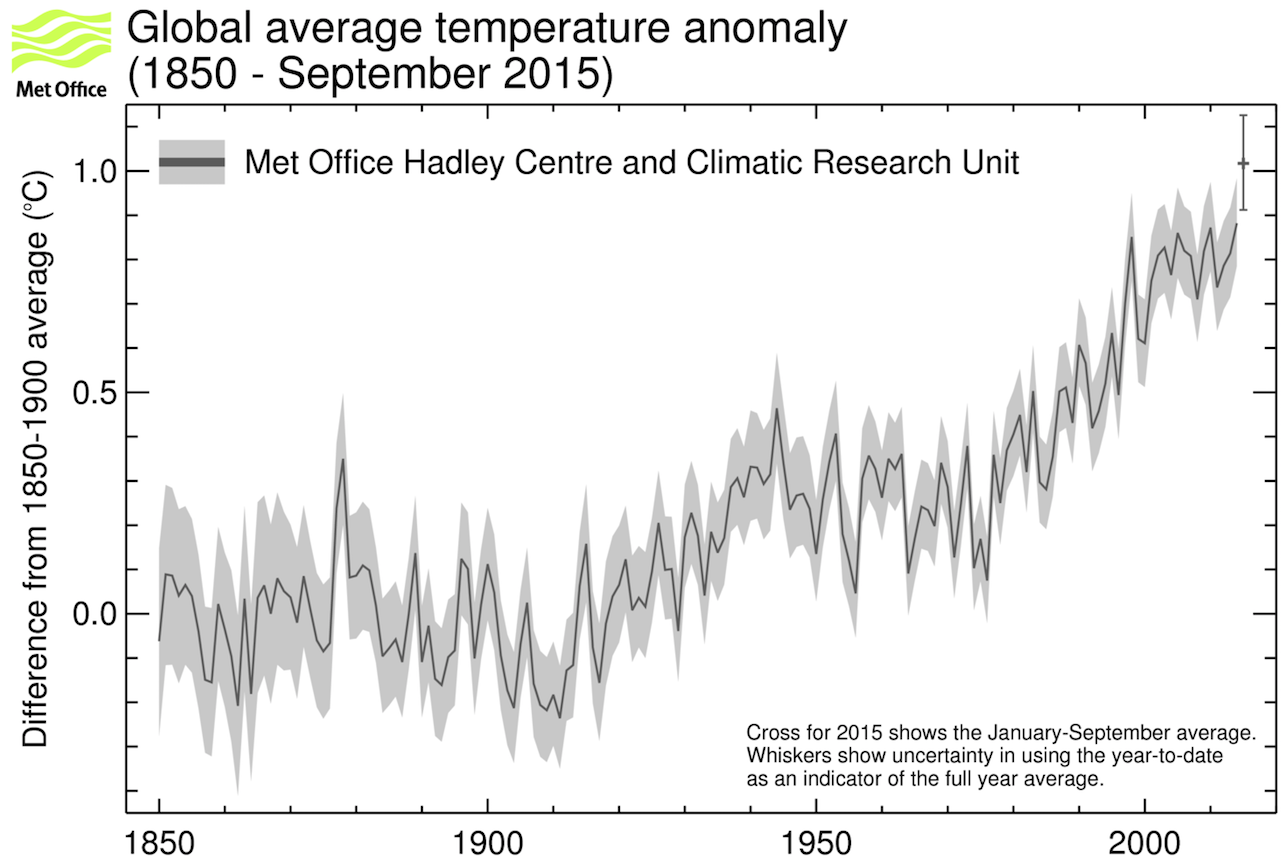
\includegraphics[width=\textwidth]{fig/L1/evolution-temperature.png}
\end{figure}
\visible<2->{\alert{Mostly known dynamical processes (based on physical principles)}}

\end{columns}
    
\end{frame}

\section{Generalities on Machine Learning}
%%%%%%%%%%%%%%%%%%%%%
\begin{frame}
\frametitle{What is this about ?}
\begin{alertblock}{Can we extract knowledge, make some predictions, determine a "model" using this large
amount of data ?}

\end{alertblock}
\pause
\begin{figure}
\begin{tikzpicture} [
	auto,
	node distance = 1cm]
	\node(H0) [anchor=east]{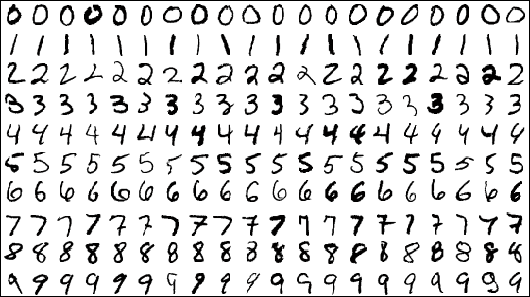
\includegraphics[width=0.4\textwidth]{./fig/L1/mnistExamples.png}};
	\node(H1) [right of =  H0, xshift = .4\textwidth]  
	{Digit \newline $\in \{0,\ldots,9\}$};
	\node(legend) [below of = H0,yshift=-4ex]{Base of images};
	\draw [very thick, ->] (H0)--(H1);
\end{tikzpicture}
\end{figure}
\pause
\begin{itemize}
\item From high dimensional data (thousands to millions dimensions) to reduced dimensional data (less than 100)
\item From disorganized data to comprehensive information
\item \alert{Can we teach a machine how to do that ?}
\end{itemize}

\end{frame}

%%%%%%%%%%%%%%%%%%%%%%%%%
\begin{frame}
\frametitle{Two classes of Machine Learning problems}
\begin{enumerate}
\item \alert{Regression}: Determination of a quantitative variable from a set of data
\begin{itemize}
\item The price of a building from various predictors (Surface, ...)
\item A physical value (Temperature, humidity, ...) in the future knowing the past
\item ...
\end{itemize}
\pause
\item \alert{Classification}: Determination of a class 
\begin{itemize}
\item A digit from a image
\item Identification of the content of an image
\item ...
\end{itemize}
\end{enumerate}
\end{frame}
%%%%%%%%%%%%%%%%%%%%%%%%%%%
\begin{frame}
\frametitle{Two types of objectives}

\begin{enumerate}[<+->]
\item \alert{Supervised learning}: we have a set of labeled data with examples of targets.
\item \alert{Unsupervised learning}: we only have unlabeled the data, we have no examples of
what we want to obtain. We want to extract a "useful" representation of these data, or
some coherent categories.
\begin{itemize}
\item Determine typical behaviors of clients in a supermarket knowing what the have bought.
\end{itemize}
\item \alert{Semi-Supervised Learning}: Only a few subset of the data are labeled
\item \alert{Reinforcement Learning}: We can initiate and observe the interaction of an agent with its environment. We want to optimize the behavior of the agent.
\begin{itemize}
\item Playing a chess game.
\end{itemize}
\end{enumerate}
\end{frame}

%%%%%%%%%%%%%%%%%%%%
\begin{frame}
\frametitle{Formally}
\begin{block}{A Machine}
\begin{equation*}
y = \mathcal{M}(x,\theta)
\end{equation*}
\begin{itemize}
\item $x$: input
\item $y$: output
\item $\mathcal{M}$: a model (named "machine")
\item $\theta$ : parameters of the model $\mathcal{M}$.
\end{itemize}
\end{block}
\alert{Machine learning} consists in optimizing $\theta$ using a set of data. 
This is the training process.
\end{frame}



%%%%%%%%%%%%%%%%%%%%
\begin{frame}
\frametitle{The Machine Learning recipe}
\begin{block}{A Machine}
\begin{equation*}
y = \mathcal{M}(x,\theta)
\end{equation*}
\end{block}
What are \alert{the ingredients}? 
\begin{columns}[t]

\column{.6\textwidth}

\begin{itemize}
    \item<2-> Some \alert{data}
    \begin{itemize}
        \item $x,y$ : supervised learning
        \item only $x$: unsupervised learning
        \item $x$ and some subset of $y$: semi-supervised learning
    \end{itemize}
    
    
    \item<3-> An \alert{objective}
        \begin{itemize}
\item $y$ is quantitative: regression
\item $y$ is a class: classification
    \end{itemize}
    \end{itemize}
    
\column{.6\textwidth}

\begin{itemize}
    \item<4-> A computational architecture (the \alert{machine})
        \begin{itemize}
        \item linear
        \item non-linear
        \item neural networks, random forest, ...
    \end{itemize}
    \item<5-> A \alert{learning} process
    \begin{itemize}
        \item Estimation of $\theta$
    \end{itemize}
\end{itemize}

\end{columns}

\end{frame}
%%%%%%%%%%%%%%%%%%
\begin{frame}{Multidimensional data}
Generally, we have multidimensional data $X$ and a one-dimensional target $y$.
\begin{figure}
\begin{tikzpicture}
\draw [fill=blue!20](0,0) rectangle (2,3);
\draw [fill=blue!20](2.5,0) rectangle (3.5,3);

\node [text centered] at (1,3.3) {features};
\node[text centered, rotate=90] at (-0.3,1.5) {samples};
\node [text centered] at (1,1.5) {\Large $X$};
\node [text centered] at (3,1.5) {\Large $y$};

  %\draw [fill=blue:20,black] (0.,0.) rectangle (1,2) ; 
\end{tikzpicture}
 \end{figure}
\end{frame}

%%%%%%%%%%%%%%%%%%%%
\begin{frame}{An illustration}
\begin{columns}
\column{.6\textwidth}
\begin{itemize}
    \item Some \alert{Data}
    \begin{figure}
    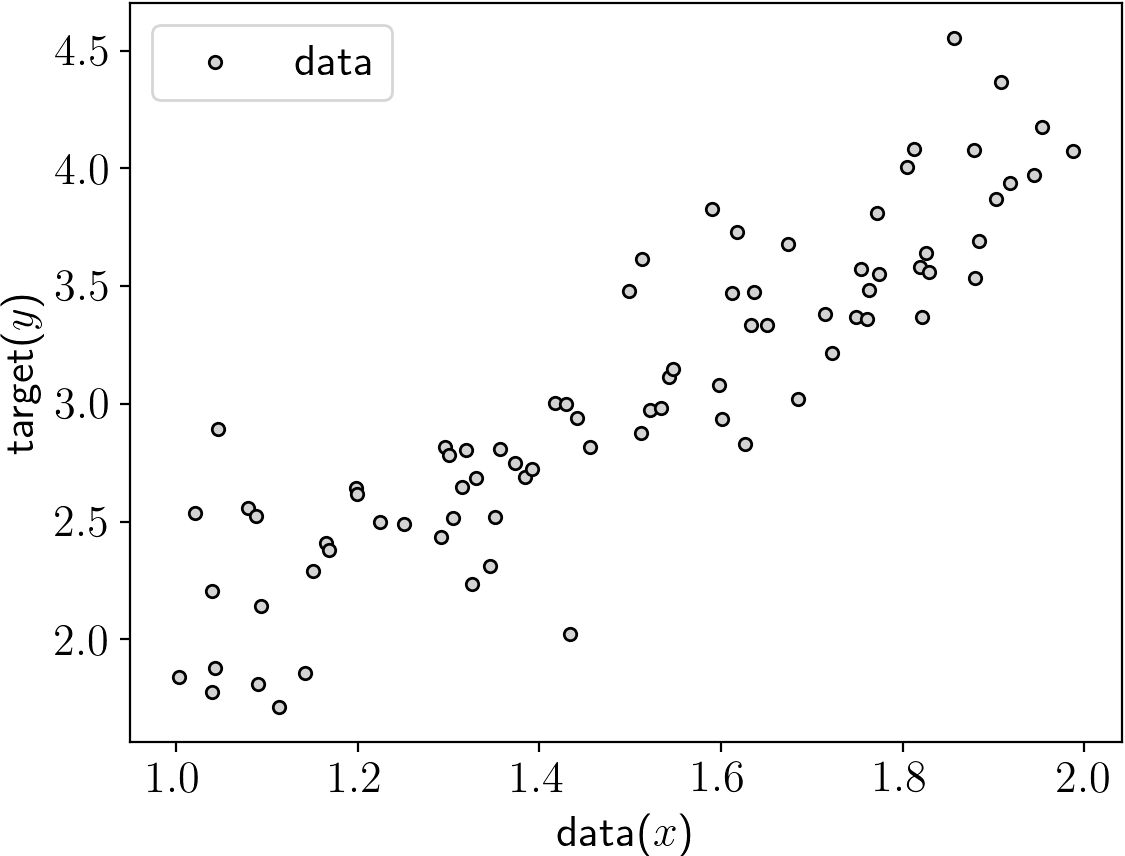
\includegraphics[width=.8\textwidth]{fig/L1/data-lin.png}
    \end{figure}

    \begin{itemize}
    \item $y$ is known: supervised learning
    \item $y$ is quantitative: regression
    \end{itemize}
\pause
\item An \alert{Objective}: Estimate $\hat{y}$ from $x$ by minimizing $(\hat{y}-{y})^2$ (Least-square objective)

\end{itemize}
\column{.5\textwidth}
\begin{itemize}
\pause
    \item A \alert{model}: $y = \theta_1 X + \theta_0$ (linear)
\pause
    \item A \alert{learning} process:
    $\mathbf{\theta}=(\mathbf{X}^T\mathbf{X})^{-1}\mathbf{X}^Ty$
\end{itemize}
\pause
\begin{block}{Result}
    \begin{figure}
    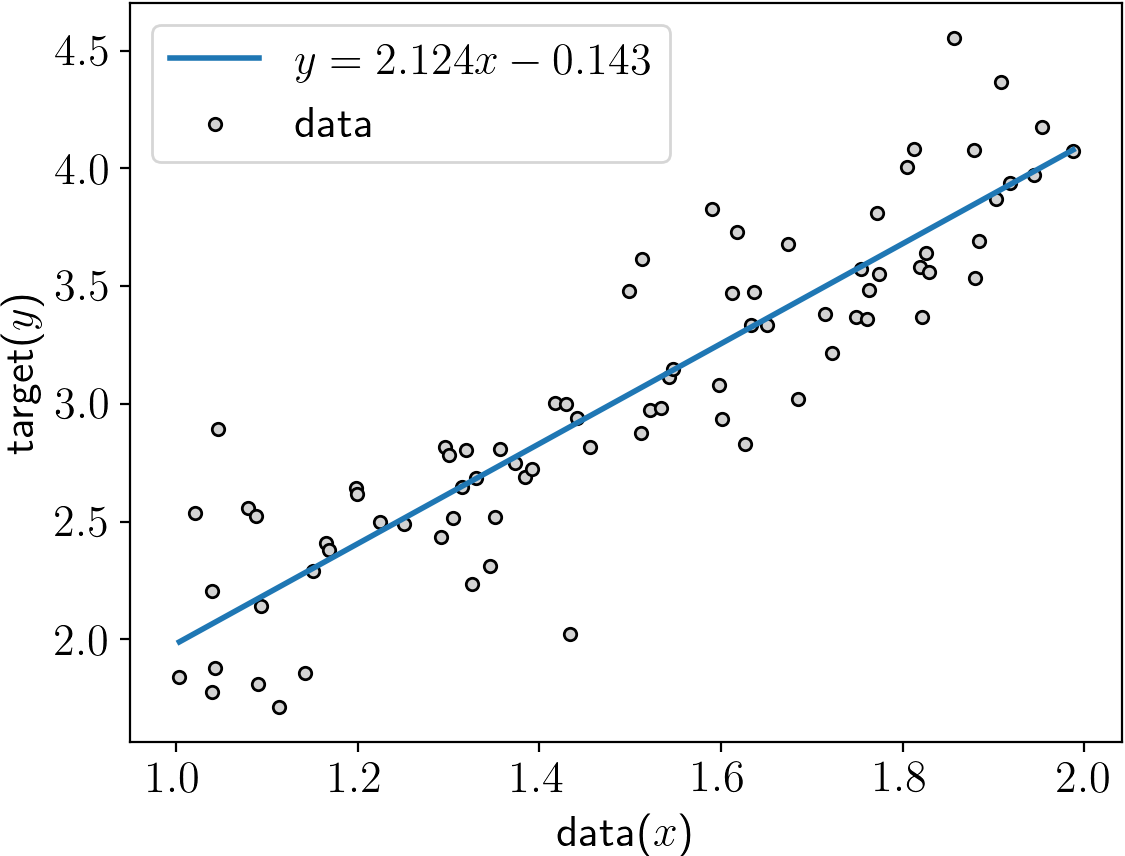
\includegraphics[width=.9\textwidth]{fig/L1/interp-lin.png}
    \end{figure}
\end{block}
\end{columns}
\end{frame}

%%%%%%%%%%%%%%%%%%%%
\section{Model selection/validation}

\begin{frame}{Choice of the model}
\begin{block}{Polynomial regression}
$y=\theta_0 + \theta_1 x + \theta_2 x^2 + \cdots + \theta_d x^d = \sum_{i=0}^d \theta_i X^i$
\end{block}
\begin{columns}
\column{.33\textwidth}
\pause
    \begin{figure}
    \caption*{degree = 1 (linear)}
    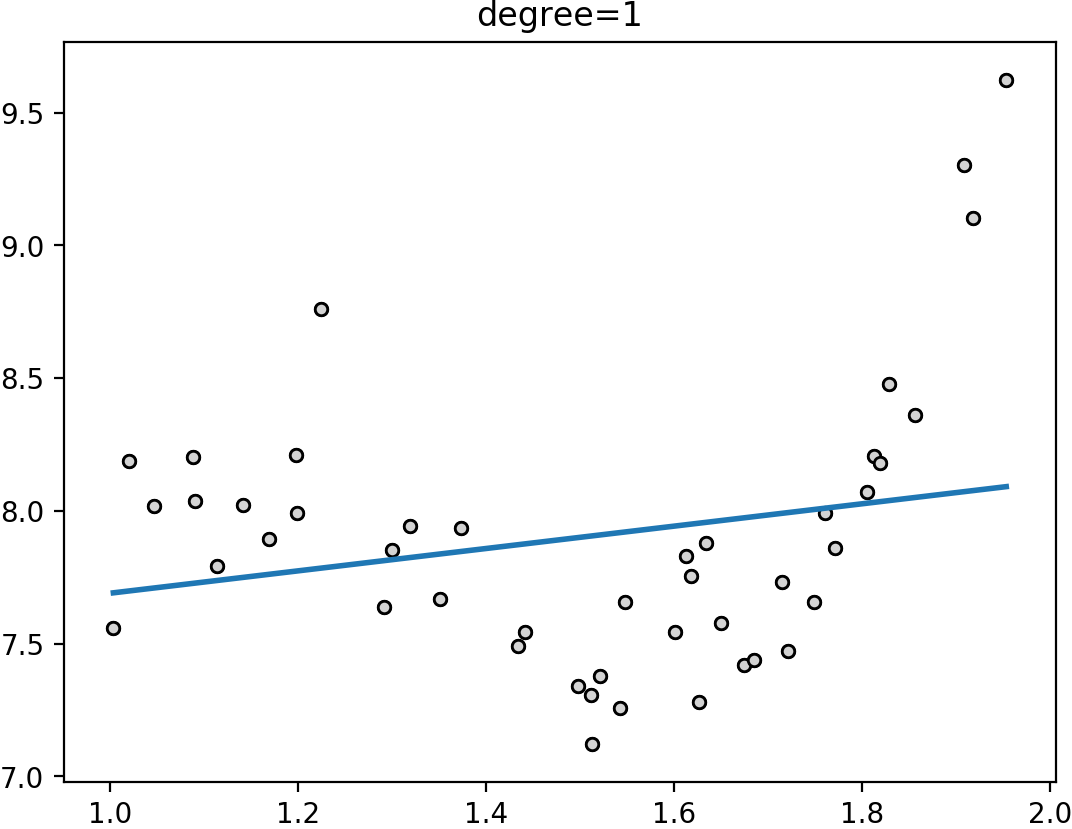
\includegraphics[width=\textwidth]{fig/L1/interp-pol-1.png}
    \end{figure}
\column{.33\textwidth}
\pause
    \begin{figure}
    \caption*{degree = 3 }
    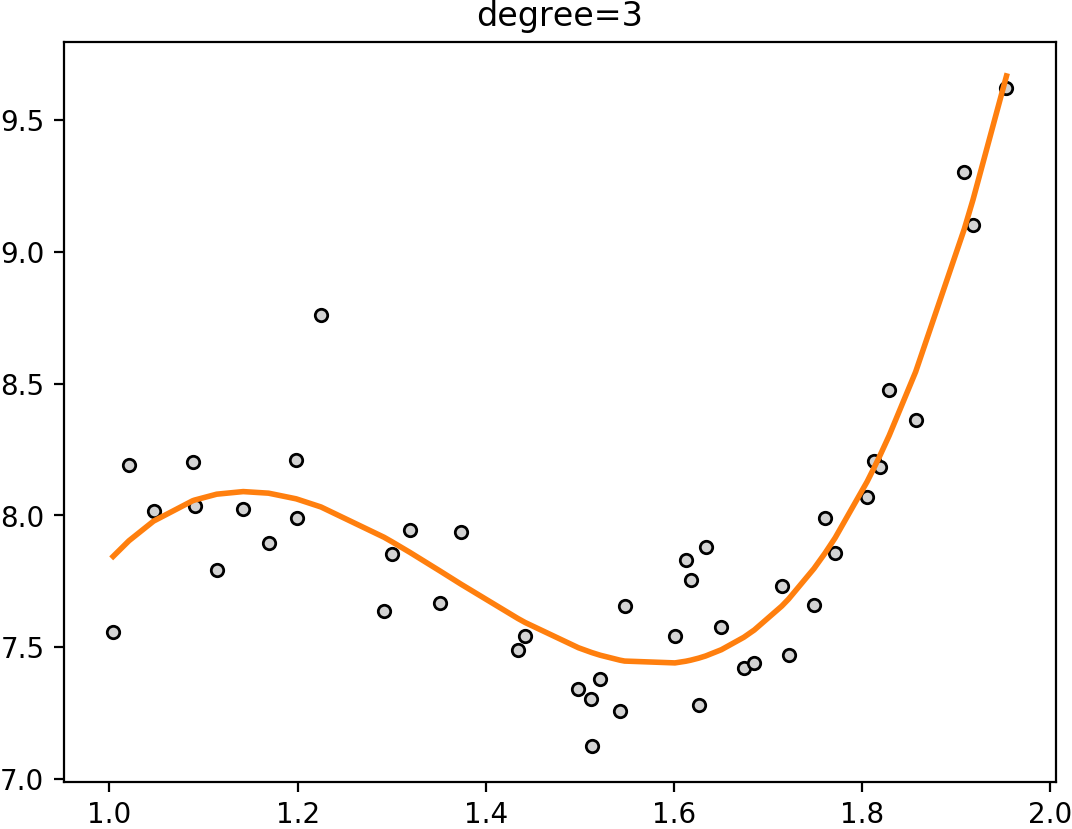
\includegraphics[width=\textwidth]{fig/L1/interp-pol-3.png}
    \end{figure}
\column{.33\textwidth}
\pause
    \begin{figure}
    \caption*{degree = 30 }
    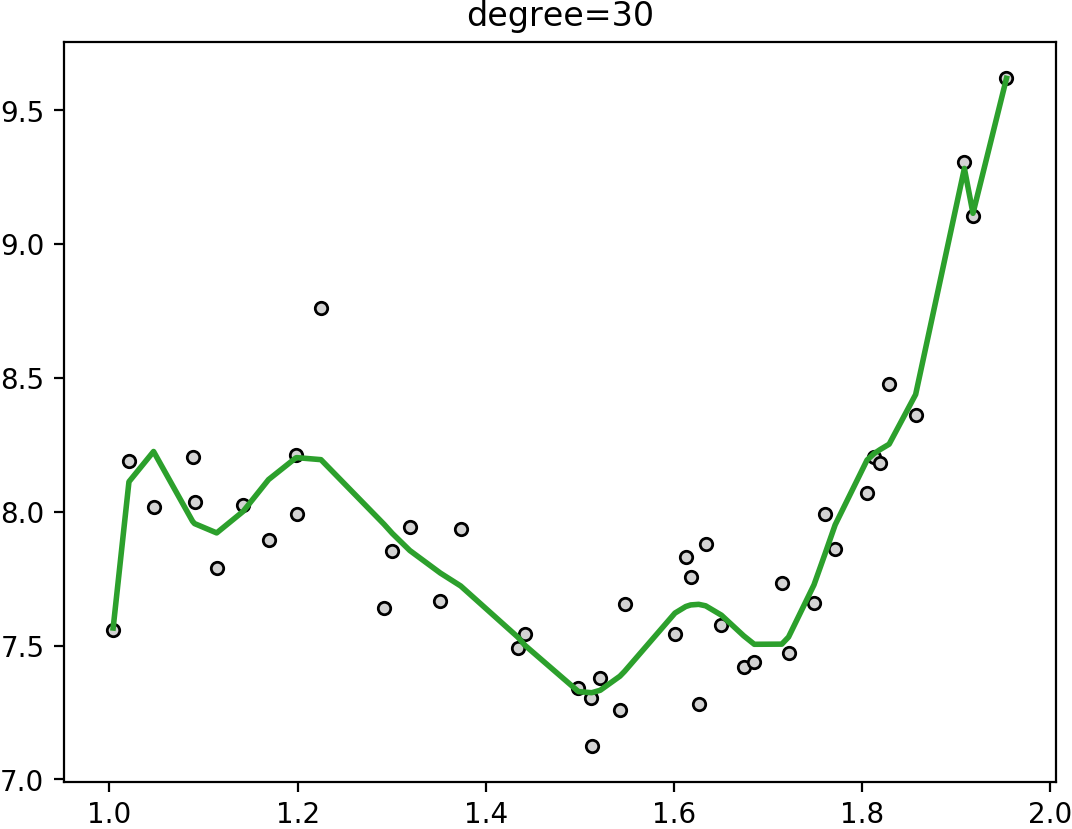
\includegraphics[width=\textwidth]{fig/L1/interp-pol-30.png}
    \end{figure}
 
\end{columns}
   
    \centering {
    \alert{What is the best model?}
    }
\end{frame}


%%%%%%%%%%%%%%%%%%%%
\begin{frame}{Train/Validation split}
\begin{block}{The idea}
Evaluate a score on a independent dataset
\end{block}
\pause
In our example we can randomly divide $(X,y)$ in two datasets:
\begin{itemize}
    \item The training dataset $X_{train},y_{train}$ used to fit the  model.
    \item The validation dataset $X_{val},y_{val}$ used to compute the score (e.g., correlation, mean-squared error)
\end{itemize}

    \begin{figure}
    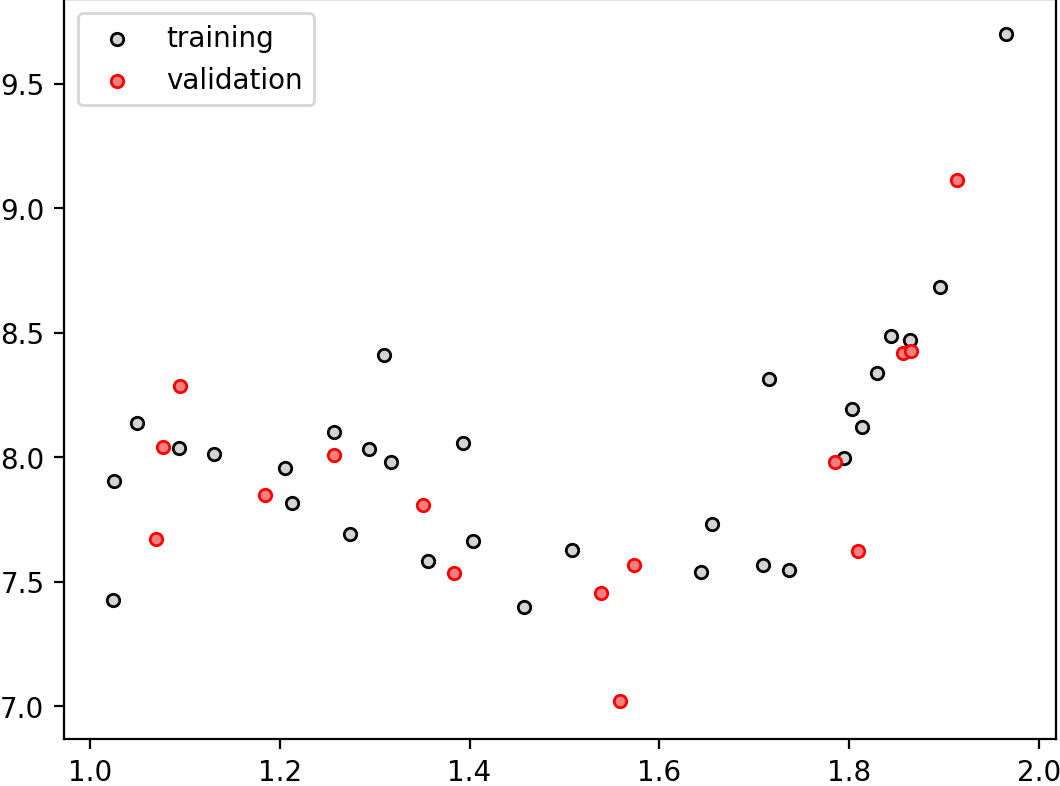
\includegraphics[width=.4\textwidth]{fig/L1/datasplit.png}
    \end{figure}

\end{frame}

%%%%%%%%%%%%%%%%%%%
\begin{frame}{Choice of the model}
\begin{columns}
\column{.5\textwidth}

    \begin{figure}
    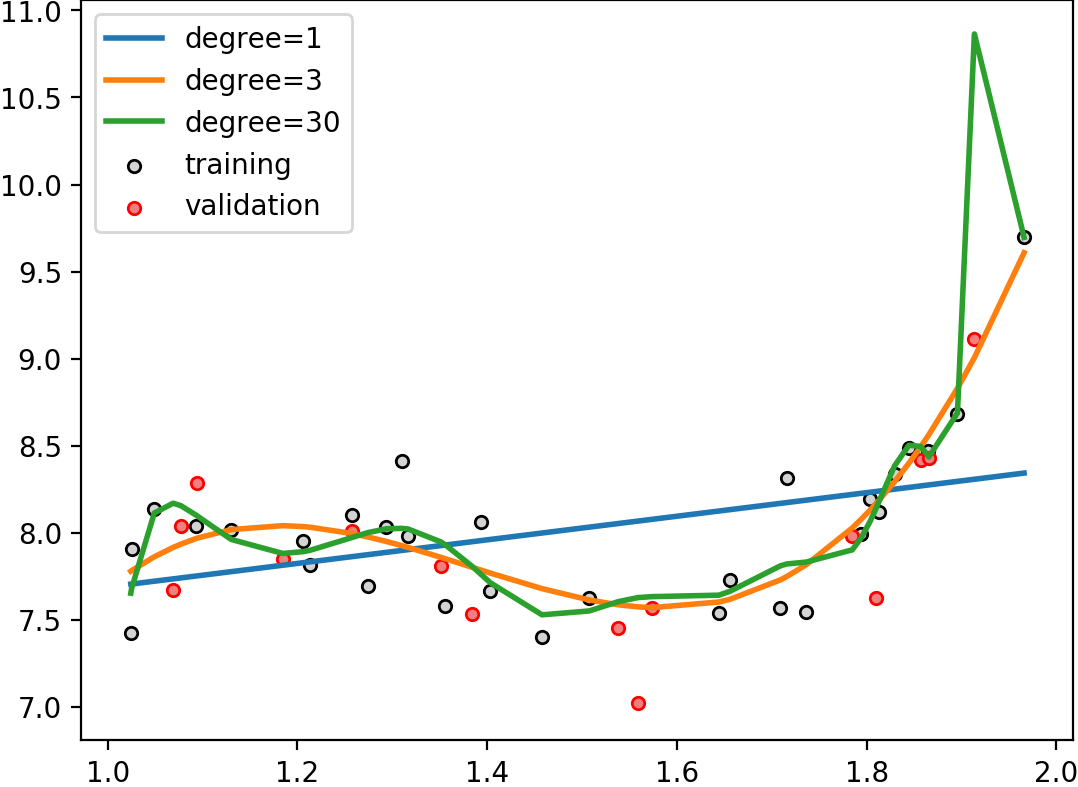
\includegraphics[width=\textwidth]{fig/L1/modelchoice.png}
    \end{figure}
\column{.5\textwidth}
Score: Mean Square Error (MSE)
\begin{table}
    \centering
    \begin{tabular}{c|c|c}
        Deg. & Train Score & Val. Score \\
        \hline
        1 & 0.17 & 0.23\\
        3 & 0.045 & 0.062\\
        30 & 0.035 & 0.27  \\
    \end{tabular}
    \end{table}
    %deg 1 ,score: val= 0.2283939842150192  , train= 0.167306864804612  , cv= 0.2768505679342689
%deg 3 ,score: val= 0.062492089527889656  , train= 0.04486320473714161  , cv= 0.05378120725339085
%deg 30 ,score: val= 0.27582336720042394  , train= 0.03473760406327127  , cv= 105306.65534552556
\end{columns}
\pause
   \begin{figure}
    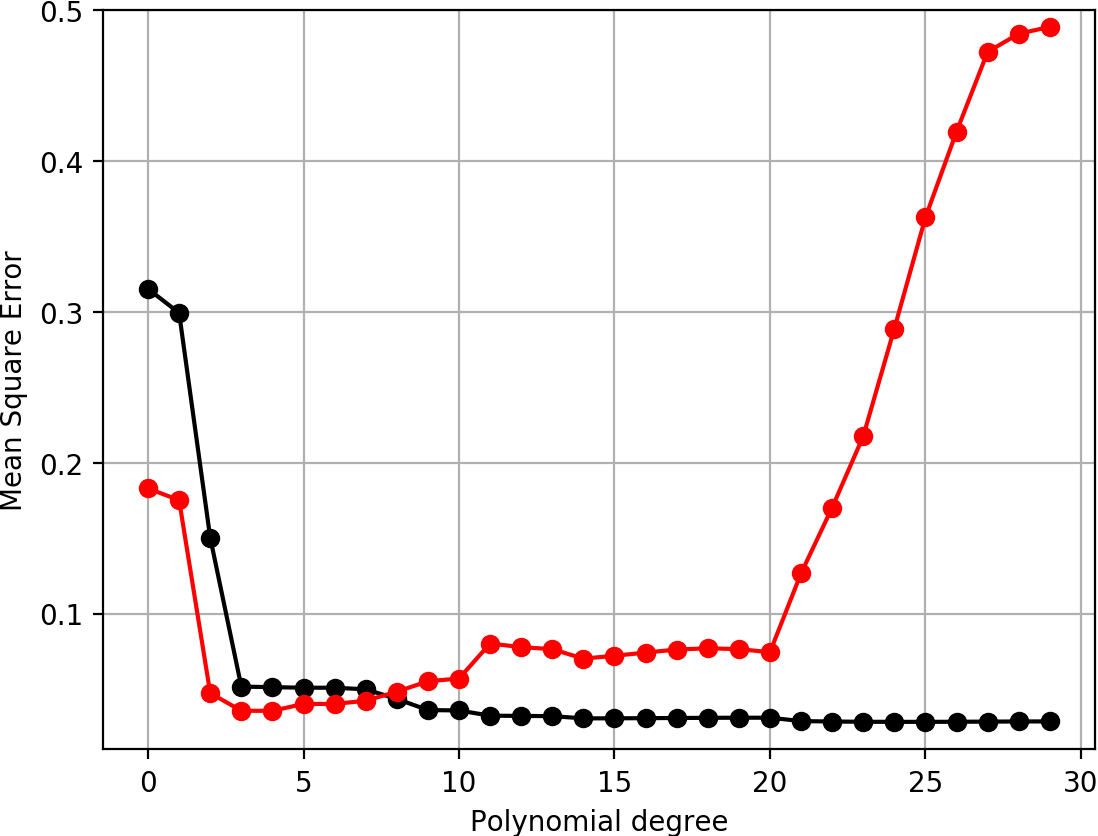
\includegraphics[width=.45\textwidth]{fig/L1/RMSE-deg-2scores.png}
    \end{figure}

\end{frame}

%%%%%%%%%%%%%%%%%%%%
\begin{frame}{Choice of the model}
\begin{block}{Polynomial regression}
$y=\theta_0 + \theta_1 x + \theta_2 x^2 + \cdots + \theta_d x^d = \sum_{i=0}^d \theta_i X^i$
\end{block}
\begin{columns}
\column{.33\textwidth}
    \begin{figure}
    \caption*{degree = 1 (linear)}
    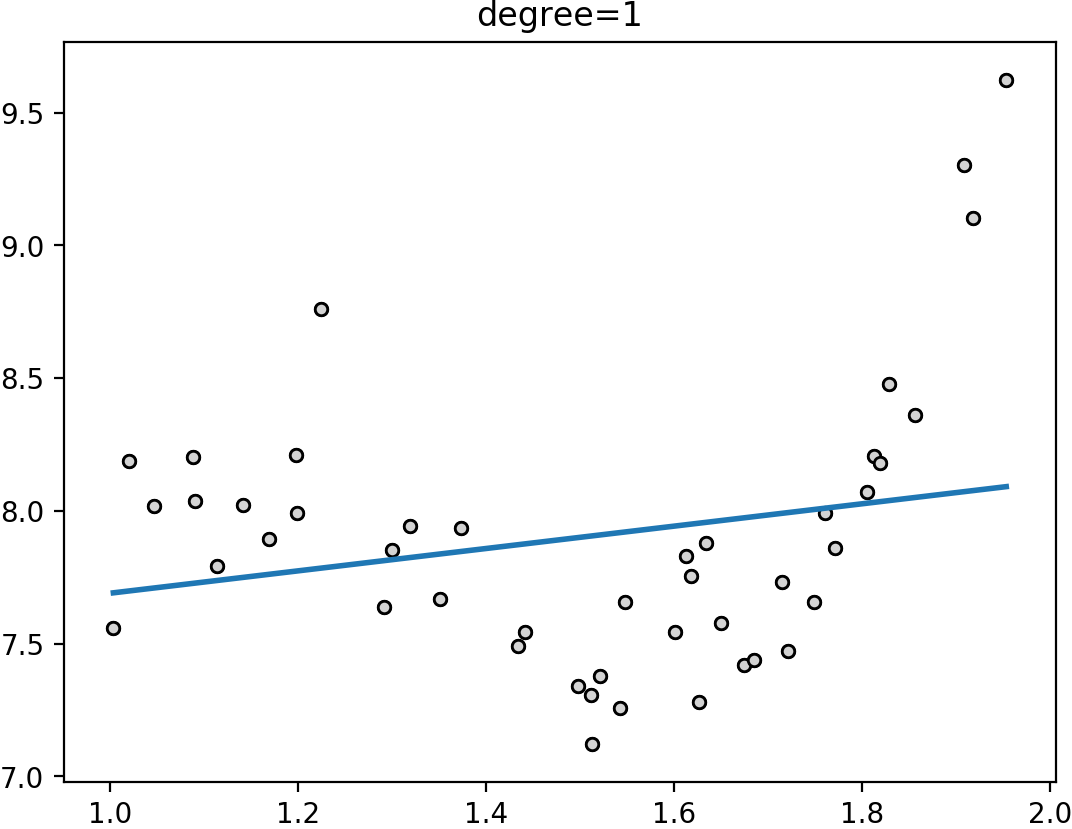
\includegraphics[width=\textwidth]{fig/L1/interp-pol-1.png}\\
        underfitting

    \end{figure}
\column{.33\textwidth}
    \begin{figure}
    \caption*{degree = 3 }
    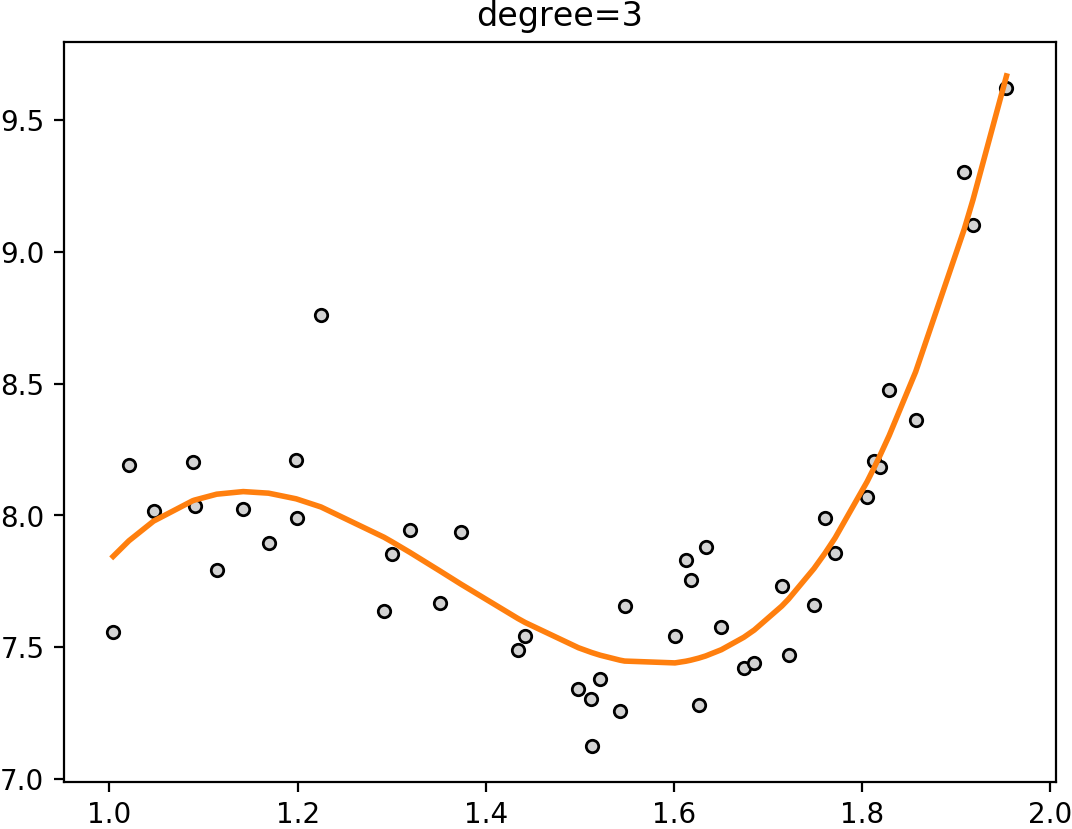
\includegraphics[width=\textwidth]{fig/L1/interp-pol-3.png}\\
        good fit

    \end{figure}
\column{.33\textwidth}
    \begin{figure}
    \caption*{degree = 30 }
    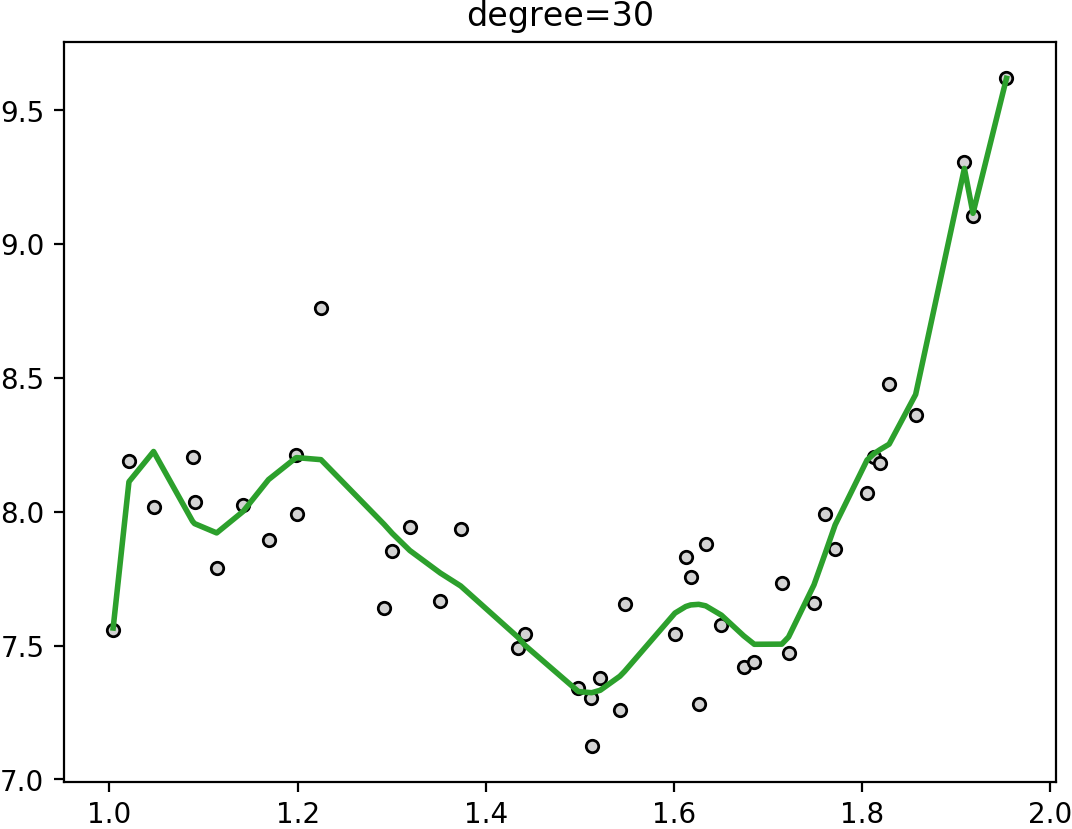
\includegraphics[width=\textwidth]{fig/L1/interp-pol-30.png}\\
        overfitting

    \end{figure}
 
\end{columns}

\end{frame}


%%%%%%%%%%%%%%%%%%%%
\begin{frame}{Train/Validation split}
     \begin{block}{Drawbacks}
\begin{itemize}
    \item drastically reduce the number of samples which can be used for learning the model
    \item Results  can depend on a particular random choice for the pair of (train, validation) sets.
\end{itemize}
\end{block}

\end{frame}
%%%%%%%%%%%%%%%%%%
\begin{frame}{More Robust: cross validation}
    \begin{block}{The idea}
    \begin{itemize}
\item Dividing the data in n folds, 
\item Learning n model (each time with a different training set),
\item Compute the mean score over n validation set.
\end{itemize}
\end{block}
   \begin{figure}
    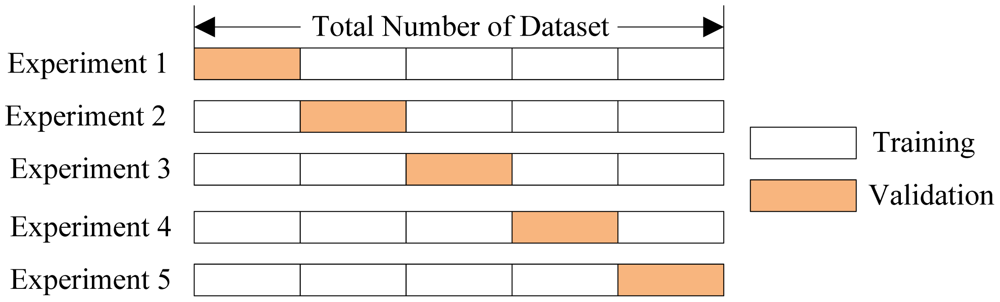
\includegraphics[width=\textwidth]{fig/L1/cv.png}
    \end{figure}

\end{frame}

%%%%%%%%%%%%%%%%%%%%
\begin{frame}{Cross-Validation}
\begin{columns}

\column{.3\textwidth}
\begin{table}
\footnotesize
    \centering
    \begin{tabular}{|c|c|}
    \hline
{\bf Fold} & {\bf MSE} \\
\hline
1 & 0.052 \\
2 & 0.043 \\
3 & 0.137 \\
4 & 0.025 \\
5 & 0.048 \\
6 & 0.144 \\
7 & 0.011 \\
8 & 0.025 \\
9 & 0.010 \\
10 & 0.028 \\
\hline
{\bf Mean} & {\bf 0.05} \\
        \hline


    \end{tabular}
    \end{table}
    
    \column{.7\textwidth}
   \begin{figure}
    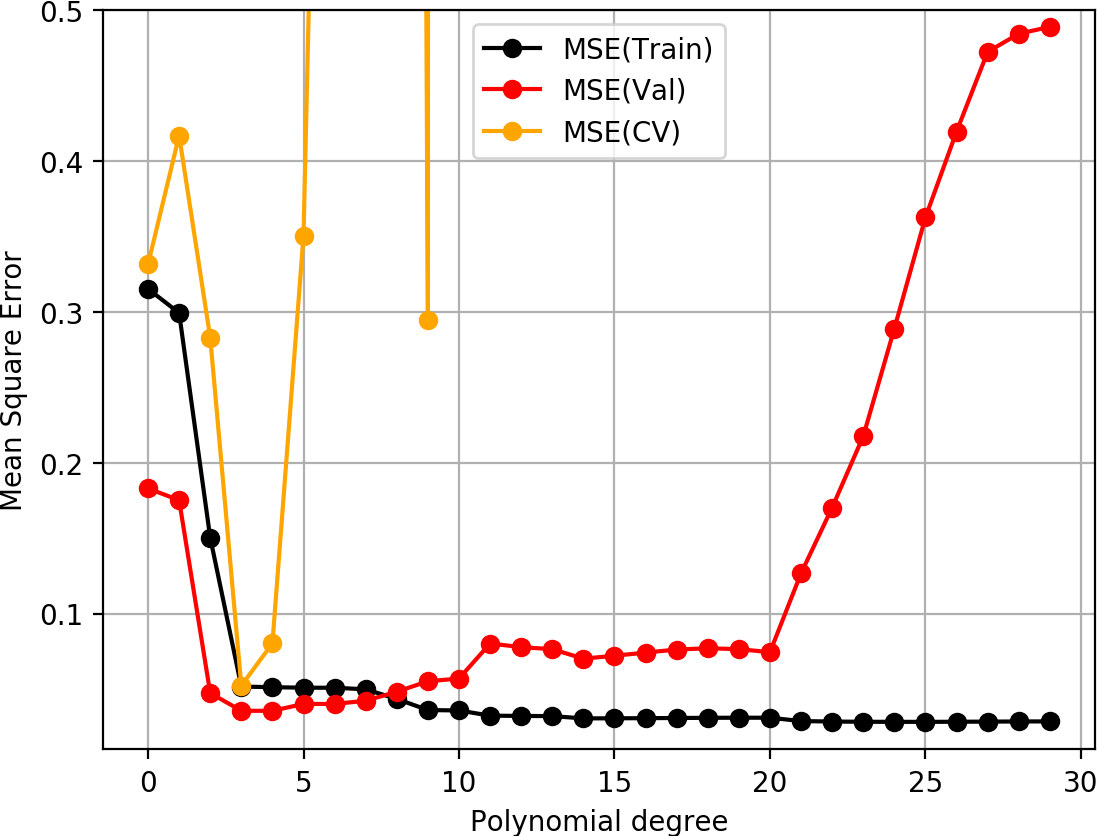
\includegraphics[width=\textwidth]{fig/L1/RMSE-deg-3scores.png}
    \end{figure}

\end{columns}

\end{frame}
%%%%%%%%%%%%%%%%
\begin{frame}{Wrapping up}
\begin{enumerate}[<+->]
    \item When applying machine learning techniques there are \alert{hyperparameters} to be determined (e.g., degree of the polynomial in polynomial regression).
    \item These \alert{hyperparameters}  can be determined by splitting the data into training/validation or by cross-validation.
    \item But then... the validation set was used to determine the best machine learning process
    \item To evaluate independanly the performance of our model, we should compute the score on a \alert{third independant dataset: The test dataset}.
    
\end{enumerate}
\end{frame}

\section{Steps of a machine learning process}

\begin{frame}{Steps}
    \begin{figure}
        \centering
     \tikzstyle{block} = [rectangle, draw, fill=blue!20, text width=7em, text centered, rounded corners, minimum height=4em]
     \tikzstyle{line} = [draw, ->]
    \tikzstyle{back} = [draw, ->, very thick, red]
     
     \begin{tikzpicture}[auto, node distance=1cm and 2cm]
     \node[block] (collect) {Collect data} ;
     
     \pause
     \node [block, below= of collect] (feature) {Preprocess /clean data\\\footnotesize{\textit{feature extractions}}};
     \path [line] (collect)--(feature);

     \pause
     \node  [block, right= of collect] (tune) {Design model};
     
     \pause
     \node  [block, right= of feature] (train) {Train model};
     \path  [line] (feature)-- node[above]{train} (train);
     \path  [line] (tune)-- (train);
     
     \pause
     \node  [block, below= of train] (evaluate) {Evaluate model};
     \path  [line] (train)--(evaluate);
     \path  [line]  (feature) --  node[above,sloped]{(cross-)valid}(evaluate);

     \pause
     \path  [back]  (evaluate) edge[bend right=80] (tune);
     \path  [back]  (evaluate) edge[bend left] (feature);
     \path  [back]  (evaluate) edge[bend right] (collect);
     
     \pause
     \node  [block, fill=red!20, left=of evaluate]  (release) {Release model};
     \path  [line]  (evaluate)--(release);
     \path  [line]  (feature) -- node[above,sloped]{test} (release);

    

     \end{tikzpicture}
    \end{figure}
\end{frame}

%%%%%%%%%%%%%%%%%%%%%%%%%%%%%%%%%%%%%%%%%%
\begin{frame}{In summary}
    From one dataset, 3 sub-datasets have to be extracted:
    \begin{itemize}
        \item A training dataset
        \item A validation dataset
    \end{itemize}
    Can be done iteratively in a cross-validation procedure.\\
    \alert {Some parameters of the model (e.g. polynomial order in a polynomial regression) were determined from the validation dataset.}
    \begin{itemize}
        \item A test dataset (independent from the two other) to estimate the final performance of the model.
    \end{itemize}
\end{frame}

%%%%%%%%%%%%%%%%%%%%%%%%%%%%%%%%%%%%%%%%%%
\section{Neural Networks}

\begin{frame}
  \frametitle{The perceptron : an artificial neuron}
  \begin{tikzpicture}[
    basic/.style={draw,fill=blue!20,text width=1em,text badly centered},
    input/.style={basic,circle},
    weights/.style={basic,rectangle},
functions/.style={basic,circle,fill=blue!10},
]
        \node[functions] (center) {};
        \node[below of=center,font=\scriptsize,text width=4em] {Activation function};
        \draw[thick] (0.5em,0.5em) -- (0,0.5em) -- (0,-0.5em) -- (-0.5em,-0.5em);
      %  \draw (0em,0.75em) -- (0em,-0.75em);
      %  \draw (0.75em,0em) -- (-0.75em,0em);
        \node[right of=center, anchor = west] (right) {$y=$ 0 ou 1};
            \path[draw,->] (center) -- (right);
        \node[functions,left=3em of center] (left) {$\sum$};
            \path[draw,->] (left) -- (center);
%        \node[weights,left=3em of left] (2) {$w_2$} -- (2) 
            \node[input,left= 4em of left] (l2) {$x_2$};
%            \path[draw,->] (l2) -- (2);
            \path[draw,->] (l2) -- node[above,midway]{$w_2$}(left);
        \node[below of=l2] (dots) {$\vdots$} ;
%(dots) node[left of=dots] (ldots) {$\vdots$};
%        \node[weights,below of=dots] (n) {$w_n$} -- (n) 
\node[input,below of=dots] (ln) {$x_n$};
%            \path[draw,->] (ln) -- (n);
            \path[draw,->] (ln) -- node[above,midway]{$w_n$}(left);
%        \node[weights,above of=2] (1) {$w_1$} -- (1) 
            \node[input,above of=l2] (l1) {$x_1$};
%            \path[draw,->] (l1) -- (1);
            \path[draw,->] (l1) -- node[above,midway]{$w_1$}(left);
%        \node[weights,above of=1] (0) {$w_0$} -- (0) 
\node[input,above of=l1] (l0) {$1$};
%            \path[draw,->] (l0) -- (0);
            \path[draw,->] (l0) -- node[above,midway]{$w_0$}(left);
        \node[below of=ln,font=\scriptsize](lin) {inputs};
        \node[right of=lin,xshift=+1em,font=\scriptsize] {weights};
    \end{tikzpicture}
\begin{block}{Computation}
$
y = f\left( w_0 + w_1. x_1 + w_2. x_2 +  \dots + w_n. x_n \right) = f\left( w_0 + \sum_{i=1}^n w_i.x_i\right)
$
\end{block}
\end{frame}

\begin{frame}{Some remarks}
\begin{itemize}[<+->]
    \item Inputs $x_i$ are the different features of the data
    \item Weight $w_i$ are the parameters of the model to optimize
    \item If the activation function is identity, it is equivalent to a linear regression
\end{itemize}
\visible<4->{
\begin{block}{}
More complexe models are build by combining several perceptrons
\end{block}
}

\end{frame}


\begin{frame}{Multi-layer perceptron (Densely connected layers)}
    \def\layersep{1.5cm}

\begin{tikzpicture}[
   shorten >=1pt,->,
   draw=black!50,
    node distance=\layersep,
    every pin edge/.style={<-,shorten <=1pt},
    neuron/.style={circle,fill=black!25,minimum size=17pt,inner sep=0pt},
    input neuron/.style={neuron, fill=green!50},
    output neuron/.style={neuron, fill=red!50},
    hidden neuron/.style={neuron, fill=blue!50},
    annot/.style={text width=4em, text centered}
]

    % Draw the input layer nodes
    \foreach \name / \y in {1,...,4}
    % This is the same as writing \foreach \name / \y in {1/1,2/2,3/3,4/4}
        \node[input neuron, pin=left:Feature \#\y] (I-\name) at (0,-\y) {};

    % set number of hidden layers
    \newcommand\Nhidden{3}

    % Draw the hidden layer nodes
    \foreach \N in {1,...,\Nhidden} {
       \foreach \y in {1,...,5} {
          \path[yshift=0.5cm]
              node[hidden neuron] (H\N-\y) at (\N*\layersep,-\y cm) {};
           }
    \node[annot,above of=H\N-1, node distance=1cm] (hl\N) {Hidden layer \N};
    }

    % Draw the output layer node
    \node[output neuron,pin={[pin edge={->}]right:Output}, right of=H\Nhidden-3] (O) {};

    % Connect every node in the input layer with every node in the
    % hidden layer.
    \foreach \source in {1,...,4}
        \foreach \dest in {1,...,5}
            \path (I-\source) edge (H1-\dest);

    % connect all hidden stuff
    \foreach [remember=\N as \lastN (initially 1)] \N in {2,...,\Nhidden}
       \foreach \source in {1,...,5}
           \foreach \dest in {1,...,5}
               \path (H\lastN-\source) edge (H\N-\dest);

    % Connect every node in the hidden layer with the output layer
    \foreach \source in {1,...,5}
        \path (H\Nhidden-\source) edge (O);

    % Annotate the layers

    \node[annot,left of=hl1] {Input layer};
    \node[annot,right of=hl\Nhidden] {Output layer};
\end{tikzpicture}
\end{frame}

\begin{frame}{More usual activation functions}
\begin{columns}
\column{.5\textwidth}
    \begin{figure}
        \centering
        Linear\\
        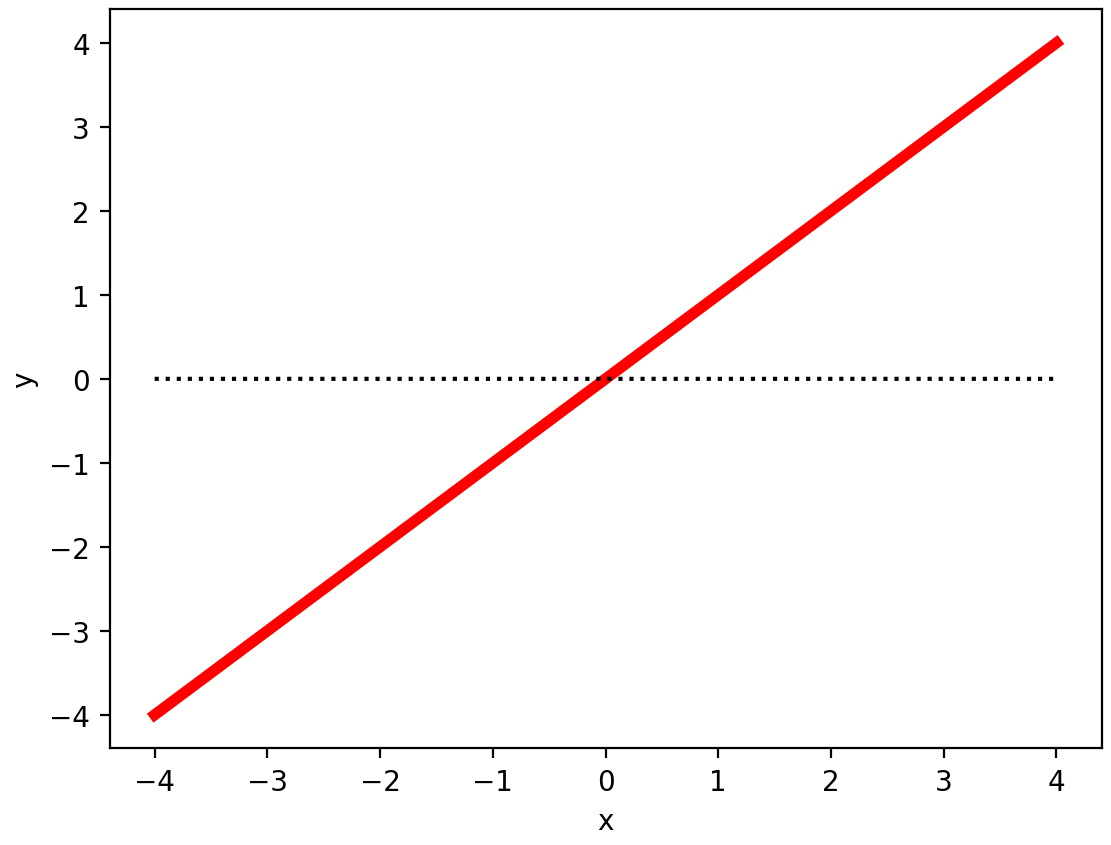
\includegraphics[width=.85\textwidth]{fig/L2/activ-linear.png}\\
        ReLU\\
        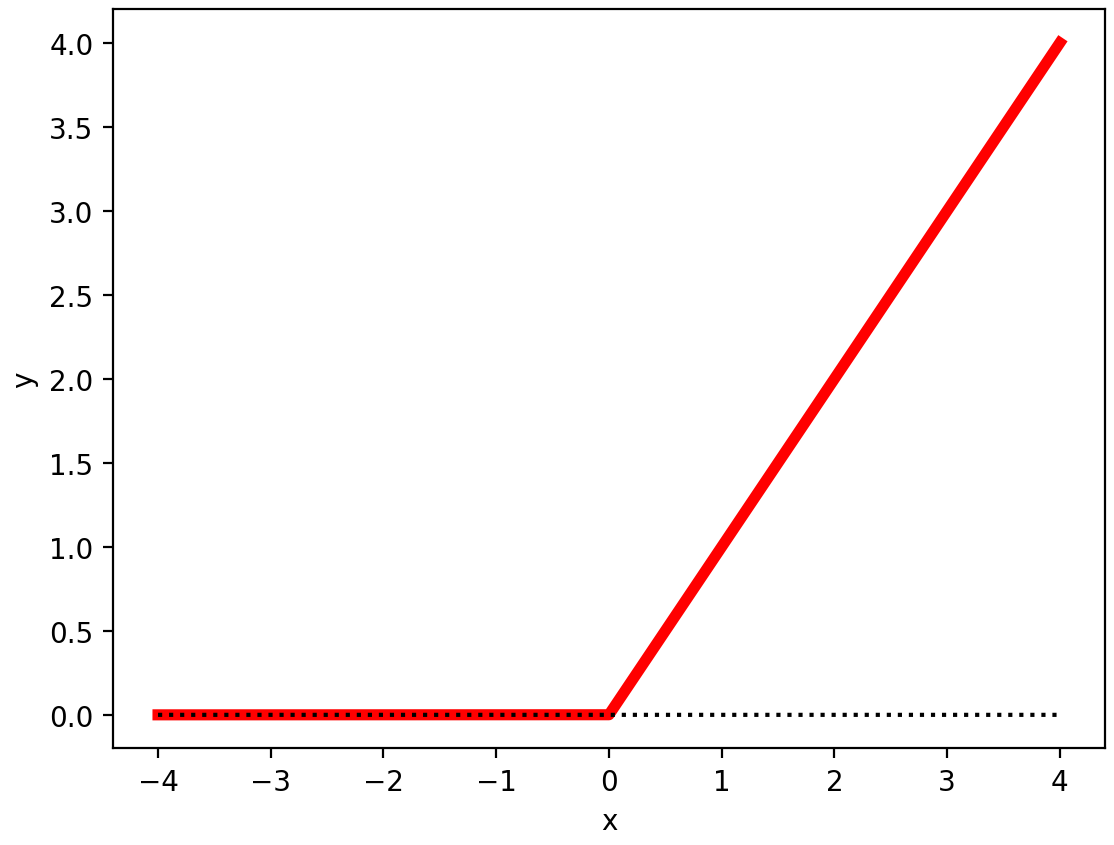
\includegraphics[width=.85\textwidth]{fig/L2/activ-relu.png}\\

    \end{figure}
\column{.5\textwidth}
    \begin{figure}
     \centering
        Hyperbolic tangent\\
        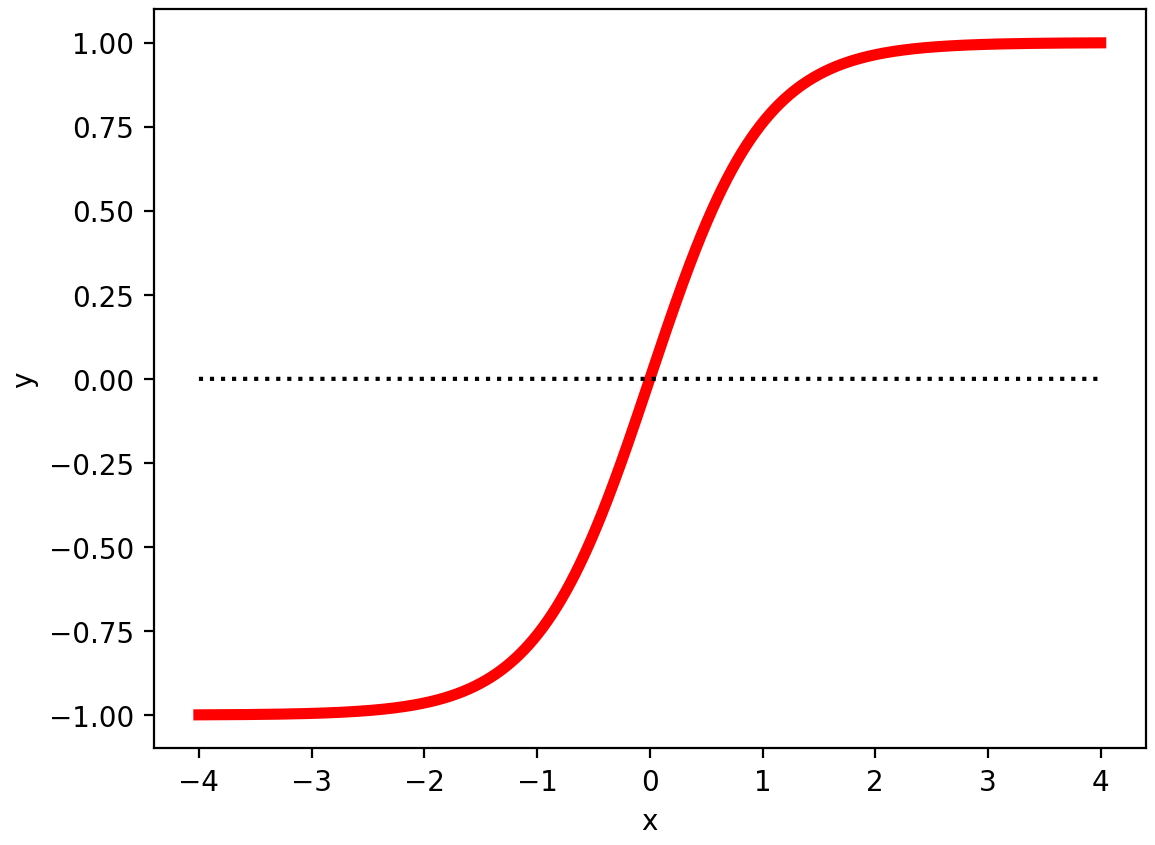
\includegraphics[width=.85\textwidth]{fig/L2/activ-tanh.png}\\
       Sigmoid\\
        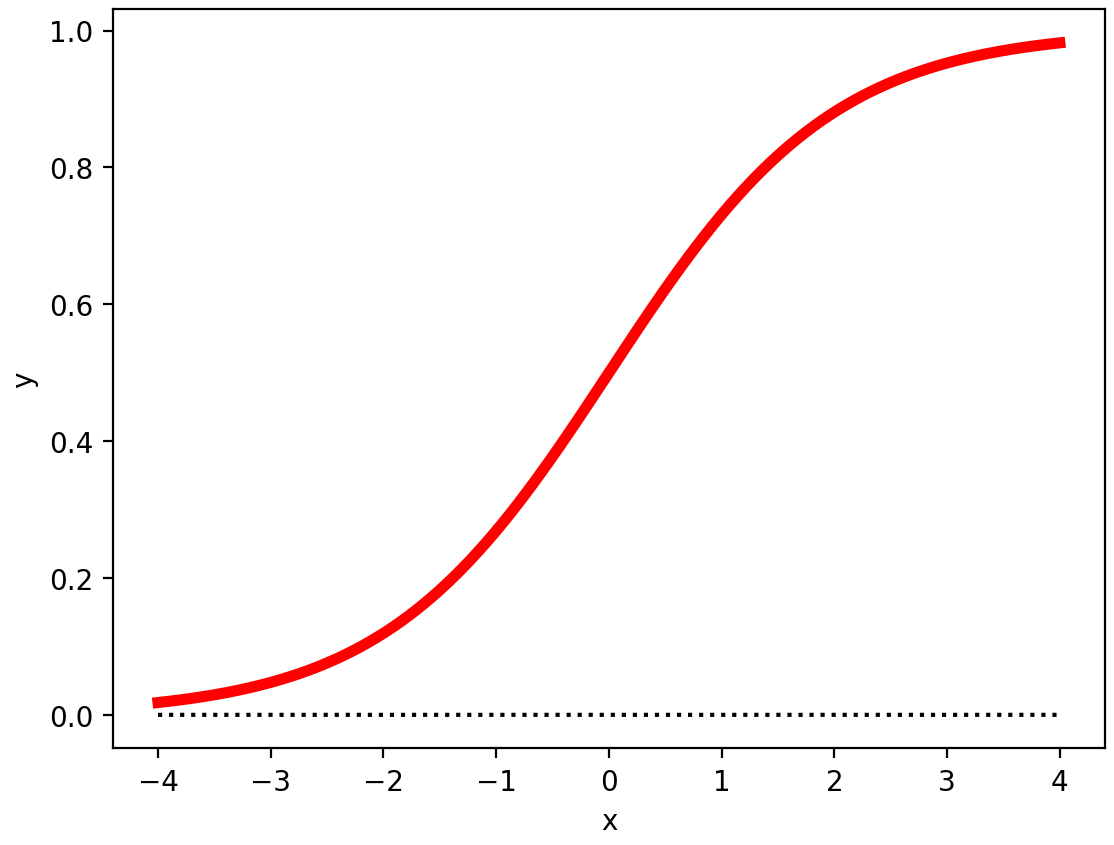
\includegraphics[width=.85\textwidth]{fig/L2/activ-sigmoid.png}\\

    \end{figure}
\end{columns}
\end{frame}


\begin{frame}{Other "fancy" activation functions}
\begin{columns}
\column{.5\textwidth}
    \begin{figure}
        \centering
        Leaky-ReLU\\
        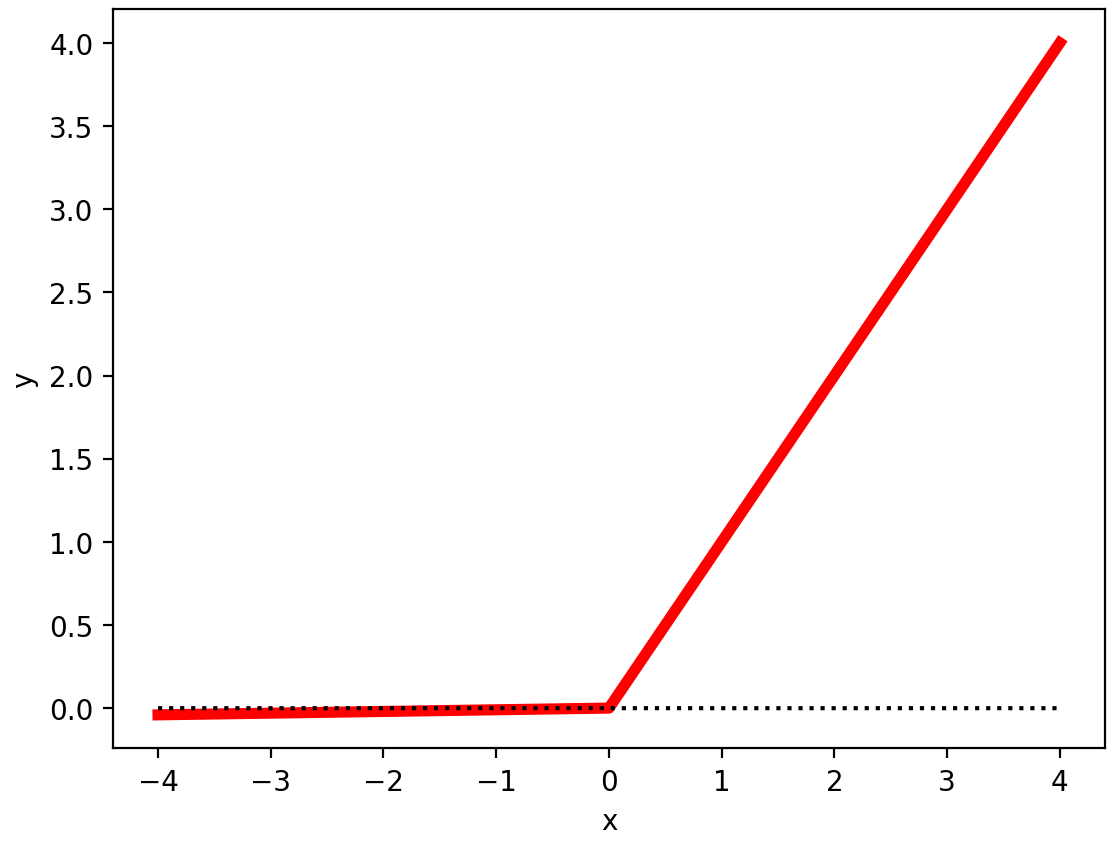
\includegraphics[width=.85\textwidth]{fig/L2/activ-l-relu.png}\\
      

    \end{figure}
\column{.5\textwidth}
    \begin{figure}
     \centering
        Swish\\
        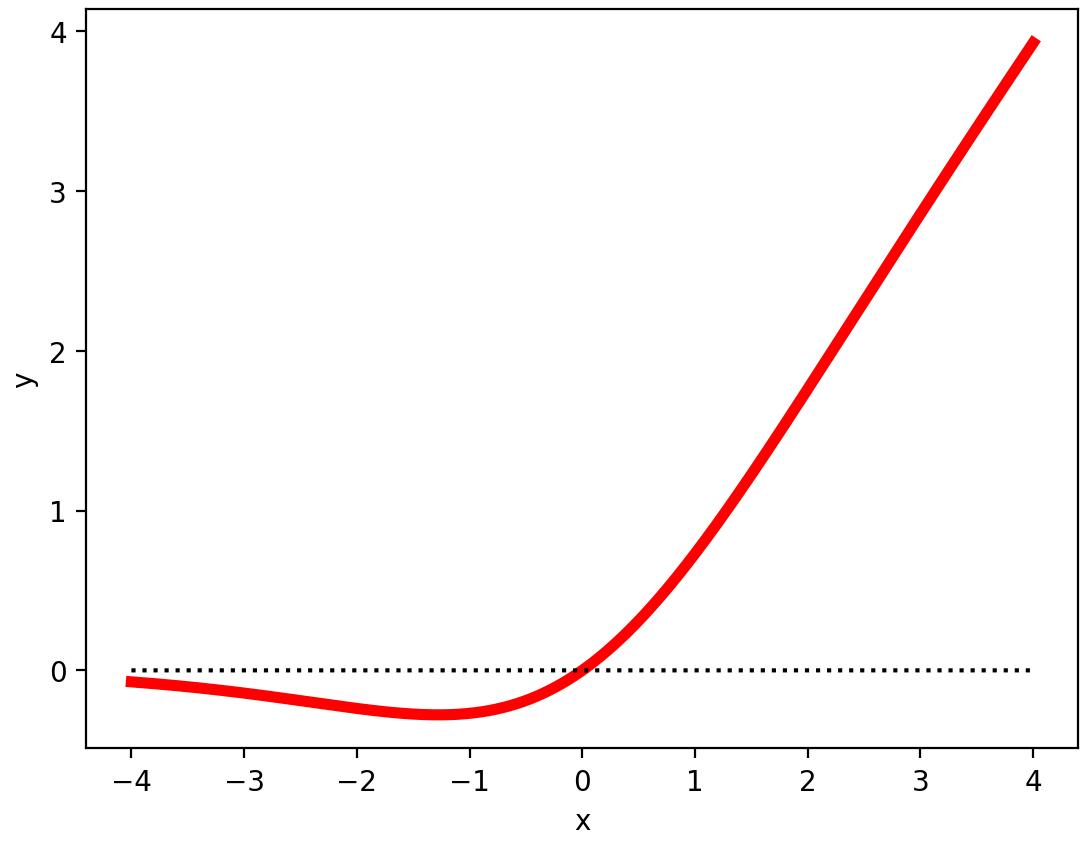
\includegraphics[width=.85\textwidth]{fig/L2/activ-swish.png}\\
     

    \end{figure}
\end{columns}
\end{frame}


\begin{frame}{Classification and regression loss}
  
   \begin{columns}
   \column{.5\textwidth}
   \alert{Regression}
   \begin{itemize}
       \item Last layer:\\
       linear or hyperbolic tangent
       \item Loss function:\\
       $$L(\hat{y},y) = \sum_i (\hat{y}_i-y_i)^2$$
   \end{itemize}
   \pause
\column{.5\textwidth}
       \alert{Classification}
   \begin{itemize}
       \item Last layer:\\
       Soft-max
       $$
       p_j=f_j(\mathbf{h}) = \frac{e^{h_j}}{\sum_k e^{h_k}}
       $$
       
       \item Loss function:\\
       Negative crossentropy
       $$L(p,y) = -\sum_i \sum_j y_{i,j}.\log{p_{i,j}}$$
   \end{itemize}
   \end{columns}
\end{frame}

\section{Gradient backpropagation}
\begin{frame}{Training a neural-net: gradient backpropagation}

\begin{columns}

\column{.5\textwidth}
\begin{figure}
    \centering
 \begin{tikzpicture}[%
    node distance = 2.5em,
    basic/.style={draw,fill=blue!20,text width=1em,text badly centered},
    input/.style={basic,circle,fill=green!20},
    output/.style={basic,circle,fill=red!20},
    weights/.style={basic,rectangle},
functions/.style={basic,circle,fill=blue!10}
]
        \node[] (center) {};
        \node[right = of center, anchor = west,output] (right) {$\hat{y}$};
        \node[above of=center,functions] (h1) {$h_1$};
        \node[below of=center,functions] (h2) {$h_2$};
        \path[draw,->] (h1) -- node[above,midway]{$w^{1}_1$}(right);
        
        \path[draw,->] (h2) --  node[below,midway]{$w^{1}_2$}(right);
        
        \node[left = of h1, input] (x1) {$x_1$};
        \node[left = of h2, input] (x2) {$x_2$};
        
        \path [draw,->] (x1) -- node[above,midway]{$w^0_{11}$} (h1);
        \path [draw,->] (x1) -- node[pos=0.25,above]{$w^0_{12}$} (h2);
        \path [draw,->] (x2) -- node[pos=0.05,above]{$w^0_{21}$} (h1);
        \path [draw,->] (x2) -- node[below,midway]{$w^0_{22}$} (h2);
\end{tikzpicture}
\end{figure}
\begin{block}{Objective}
Determination of the best set of weights $\mathbf{w}$ to minimize the Loss function $L(\mathbf{w}) = ||\hat{y}(\mathbf{w})-y||^2$.\
\alert{Calculation of $\partial L/\partial w$}
\end{block}
\column{.6\textwidth}
\begin{enumerate}[<+->]
    \item Given a couple $(x,y)$
    \item \alert{Forward computation:}\\
    $h_j  =  f_0(\sum_{i=1}^2 w^0_{ij}.x_i)$\\
$\hat{y}  =  f_1(\sum_{j=1}^2 w^1_j. h_j)$
\item \alert{Compute the gradient of the loss:~}
$\boxed{\color{red}\partial L/\partial \hat{y}}$

    \item \alert{Gradient Backpropagation:}
    \begin{itemize}
   \item Layer 1\\
   $\alert{\partial L/\partial w_j^1} = 
   \boxed{\color{red}\partial L/\partial \hat{y}}.
   \partial f_1 / \partial w^1_j$\\
   
   $ \boxed{\color{blue}\partial L/\partial h_j} = 
    \boxed{\color{red}\partial L/\partial \hat{y}}. 
   \partial f_1 / \partial h_j$
   
   \item Layer 0\\
   $\alert{\partial L/\partial w^0_{ij}}=
  \boxed{\color{blue}\partial L/\partial h_j}
   .\partial f_1 / \partial w^0_{ij}  $
    
    \end{itemize}
\end{enumerate}

\end{columns}

\end{frame}

\section{Optimizing a machine learning (gradient method)}

\begin{frame}{Optimizing the loss}
    Several loss function (depending on the problem) can be defined.
    
    For example, Mean Square Error:
    
    \begin{alertblock}{Method}
    Find a minimum of L by adjustig the parameters (weights) $\mathbf{w}$ given the gradient of the loss with respect to the weights $\nabla_\mathbf{w}L$.
    \end{alertblock}
\end{frame}



\begin{frame}{Batch Vs Stochastic training}
Dataset: $(X,Y)$ with N samples denoted $(\mathbf{x_i},y_i)$

\begin{columns}[t]
\column{.56\textwidth}
\begin{footnotesize}
\begin{block}{Batch gradient:}\end{block}
    \begin{algorithmic}
    \Require{Learning rate(s): $\nu_k$}
    \Require{Initial weights: $\mathbf{w}$}
    \State $k \leftarrow 1$
    \While {stopping criterion not met}
   % \Require{NNNN}
    %\State Sample $m$ examples ($\mathbf{x}_i,y_i)$ from ($X,y$)
    \State Compute gradient: $\mathbf{g} \leftarrow \frac{1}{N}\sum_i^N\nabla_\mathbf{w}L(f(\mathbf{x}_i,y_i))$
    \State Update weights: $\mathbf{w} \leftarrow \mathbf{w} - \nu_k\mathbf{g}$
    \State $k \leftarrow k + 1$
    \EndWhile 
    \end{algorithmic}
    \end{footnotesize}
    \alert{1 Update / N forwards}
    \pause
    \column{.56\textwidth}
\begin{footnotesize}
\begin{block}{Stochastic gradient:}\end{block}
    \begin{algorithmic}
    \Require{Learning rate(s): $\nu_k$}
    \Require{Initial weights: $\mathbf{w}$}
    \State $k \leftarrow 1$
    \While {stopping criterion not met}
   % \Require{NNNN}
    %\State Sample $m$ examples ($\mathbf{x}_i,y_i)$ from ($X,y$)
    \State Sample an example ($\mathbf{x},y)$ from ($X,Y$)
    \State Compute gradient: $\mathbf{g} \leftarrow \nabla_\mathbf{w}L(f(\mathbf{x},y))$
    \State Update weights: $\mathbf{w} \leftarrow \mathbf{w} - \nu_k\mathbf{g}$
    \State $k \leftarrow k + 1$
    \EndWhile 
    \end{algorithmic}
    \end{footnotesize}
    \alert{1 Update / 1 forward}
    
    
    \end{columns}
\end{frame}

\begin{frame}{Mini-Batch training}
Dataset: $(X,y)$ with N samples
\begin{footnotesize}
\begin{block}{Mini-Batch gradient:}\end{block}

    \begin{algorithmic}
    \Require{Learning rate(s): $\nu_k$}
    \Require{Initial weights: $\mathbf{w}$}
    \State $k \leftarrow 1$
    \While {stopping criterion not met}
   % \Require{NNNN}
    \State Sample $m$ examples ($\mathbf{x}_i,y_i)$ from ($X,y$)
    \State Compute gradient: $\mathbf{g} \leftarrow \frac{1}{m}\sum_i^m\nabla_\mathbf{w}L(f(\mathbf{x}_i,y_i)$
    \State Update weights: $\mathbf{w} \leftarrow \mathbf{w} - \nu_k\mathbf{g}$
    \State $k \leftarrow k + 1$
    \EndWhile 
    
    \end{algorithmic}
    \end{footnotesize}
    \pause
        \alert{$m$ Update / 1 forward}\\
        $m=1$: Pure stochastic gradient.\\
        $m=N$: Batch gradient

\end{frame}

%%%%%%%%%%%%%%%%%%%%%%%%%%%%%%%%%%%%%%%%%%%%%%
\section{A quick typology of few neural nets}
%%%%%%%%%%%%%%%%%%%%%%%%%%%%%%%%%%%%%%%%%%%%%%

\begin{frame}{Convolutional neural networks}
    
\end{frame}
%%%%%%%%%%%%%%%%%%%%%
\begin{frame}{Recurrent Neural Networks}
    \begin{figure}
        \centering
        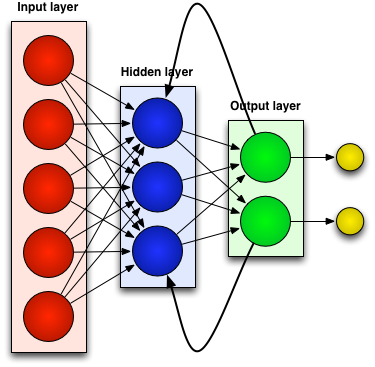
\includegraphics[width=.4\textwidth]{fig/L2/rnn.png}

    \end{figure}

Some popular types of recurrent neural networks:
\begin{itemize}
    \item Long short-term memory (LSTM)
    \item Gated Reccurent Unit (GRU)
\end{itemize}
\alert{Used in machine translation and text processing}
\end{frame}

\begin{frame}{Autoencoders}
    \begin{figure}
        \centering
        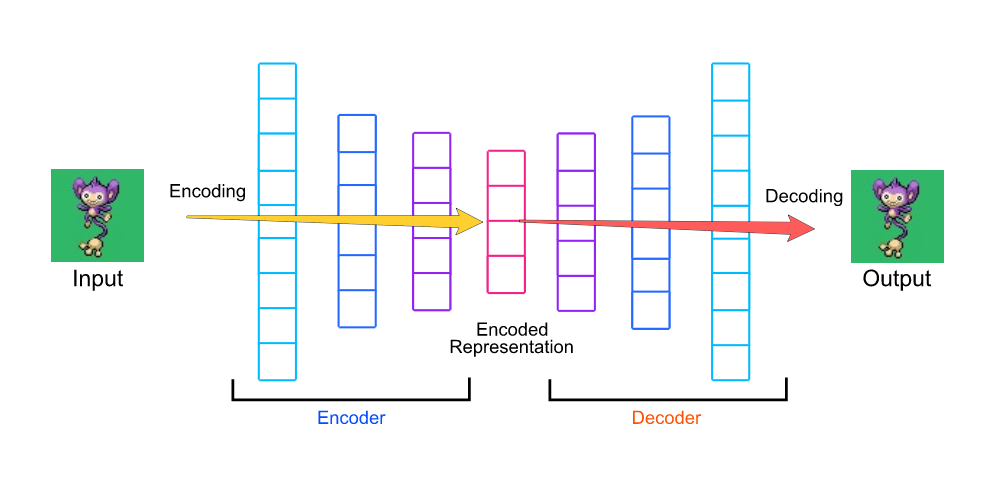
\includegraphics[width=.9\textwidth]{fig/L2/AE.png}

    \end{figure}
\alert{Used in image denoising, compressing, generation,...}
    
\end{frame}

\begin{frame}{Generative adversarial networks}
    \begin{figure}
        \centering
    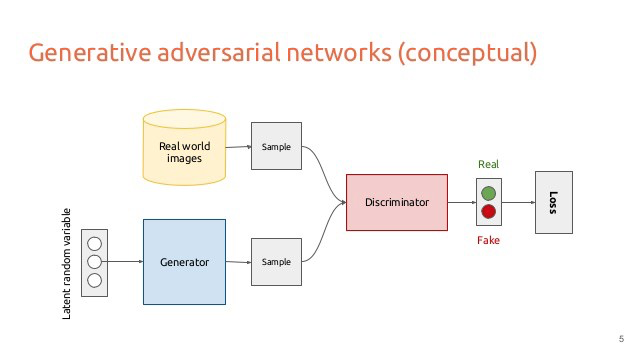
\includegraphics[width=.9\textwidth]{fig/L2/GAN.png}
  \end{figure}
    
\end{frame}

\begin{frame}{Residual Networks}
    \begin{columns}
    \column{.5\textwidth}
        \begin{figure}
        \centering
        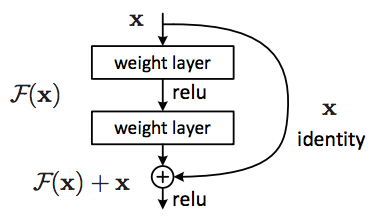
\includegraphics[width=.9\textwidth]{fig/L2/res_block.png}

    \end{figure}
    $x$~: input, $y$~: output
    $$
    y = x + \mathcal{F}(x) 
    $$
    \pause
    \column{.5\textwidth}
            \begin{figure}
        \centering
        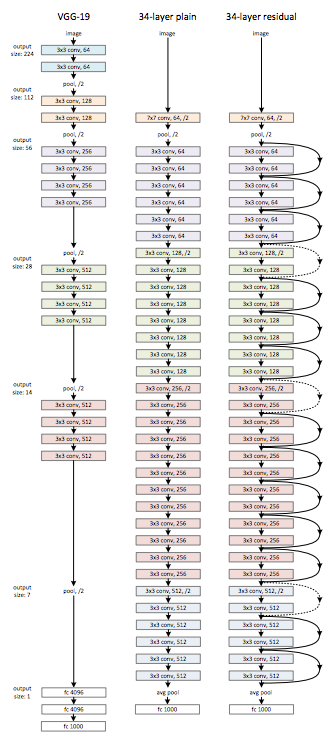
\includegraphics[height=.9\textheight,trim={4cm 0cm 0cm 0cm},clip]{fig/L2/resnet_full.png}

    \end{figure}
    \end{columns}
\end{frame}



\end{document}